%%%%%%%%%%%%%%%%%%%%%%%%%%%%%%%%%%%%%%%%%%%%%%%%%%%%%%%
%%                 TSE design margins                %%
%%%%%%%%%%%%%%%%%%%%%%%%%%%%%%%%%%%%%%%%%%%%%%%%%%%%%%%
\chapter{Design margin quantification and optimization}
\chaptermark{Design margin quantification and optimization}
\label{ch:TSEcont}
%%%%%%%%%%%%%%%%%%%%%%%%%%%%%%%%%%%%%%%%%%%%%%%%%%%%%%%

This chapter describes a novel design tool for quantifying the level of overdesign in a product via the notion of excess and buffer which constitute the design margins. These definitions are quantified in a multi-dimensional parameters space using rigorous mathematical tools. Design margins determine the product's capacity for absorbing change and therefore its robustness. However, excessive margins result in overdesign and severe operational costs.

We therefore develop a design methodology for strategically allocating design margins without compromising the product's reliability and ability to meet uncertain requirements.

The methodology in this chapter is demonstrated using an industrial case study for the remanufacturing of a \ac{TRS}. The thermomechanical model described in Section~\ref{sec:thermomech} along with the load case in Section~\ref{subsec:thermalloadcase} is used to define the design variables and uncertain parameters involved in the remanufacturing design problem. Remanufacturing is performed by \ac{AM} using laser \ac{DED}. The design space considered in this problem is finite since the decision variables are categorical. This kind of problem was chosen to show importance of high level conceptual decisions on the performance of a design as requirements change gradually.

We begin by defining the methodology for obtaining the set-based solutions for arbitrary design and parameters spaces in Section~\ref{sec:TSEmethods}. We then demonstrate the methodology for the remanufacturing of the \ac{TRS} in Section~\ref{sec:TSEcasestudy}. We present the corresponding results in Section~\ref{sec:TSEresults}. We provide some insights and conclusions about the uses and limitations of the developed framework in Section~\ref{sec:TSEcontsummary}.

%============================ METHODOLOGY ============================%
\section{Methodology} \label{sec:TSEmethods}

We consider a product design problem where requirements change several times throughout the product's lifecycle or development process. In this chapter, we will refer to these two time periods as the product cycle for conciseness. Requirements changes occur after a defined period of time (referred to as an epoch) has elapsed.

A decision regarding product redesign is made at the beginning of each epoch depending on a number of factors. The factors driving these decisions include capability, buffer, excess, and reliability. We will formally define these terms.

%---------------------------------------------------------------------%
% Mathematical definitions
\subsection{Mathematical formulation of design metrics} \label{subsec:designmetrics}

The parameters space in which our design metrics are defined is the set of values assumed by the uncertain parameters driving the requirements and feasibility criteria. The parameters vector $\mathbf{p} = \left[p_1 ~ p_2 ~ \cdots ~ p_n\right]^{\mathrm{T}}$ is defined in the multi-dimensional parameters space $\mathbf{p}\in\mathbb{R}^n$, where $n$ is the number of uncertain parameters.

Capability is defined as the set of possible values for a design parameter for which feasibility is maintained \cite{Eckert2019}. The feasibility criteria are imposed as a set of constraints that the design must satisfy $\mathbf{g}_{f}(\mathbf{p}) - \mathbf{t} \le 0$, where $\mathbf{t}$ is a vector of threshold values that the constraint function $\mathbf{g}_{f}(\mathbf{p})$ must exceed. Unlike requirements, feasibility constraints are fixed throughout the product cycle. The set defining capability is given by the following definition.

\begin{equation} \label{eq:capability}
	\textit{C} = \left\{\mathbf{p} \in \mathbb{R}^n~|~\mathbf{g}_{f}(\mathbf{p}) - \mathbf{t} \le 0\right\}.
\end{equation}

In engineering problems, such constraints may be obtained from computational models instead of analytical expressions. In order to alleviate the computational effort used to classify regions of the parameters space into capability, buffer, and excess, a surrogate may be used.

We represent requirements using a joint \acf{PDF} $F_{\mathbf{X}}\left(\mathbf{p}\right)$ as was done in the literature \cite{Villanueva2014,Pradlwarter2005,Frangopol2003a,Zhu2013a}. This method has the advantage of being able to specify requirements in a multi-dimensional parameters space. $F_{\mathbf{X}}\left(\mathbf{p}\right)$ could be any kind of \ac{PDF} such as Gaussian or uniform distributions and describes the distribution of the uncertain parameters.

Knowing the capability of a design and the corresponding requirement joint \ac{PDF}, we can calculate reliability in terms of the probability that the design satisfies the requirement \cite{ForouzandehShahraki2014,Bucher2009}. The probability is calculated from the joint \ac{PDF} such that a value for the uncertain parameter sampled from $F_{\mathbf{X}}\left(\mathbf{p}\right)$ lies within the capability set $C$. This probability value represents reliability of the design $\mathbb{P}(\mathbf{p} \in C)$. Reliability is defined by the following expression.

\begin{equation} \label{eq:reliability}
	\mathbb{P}(\mathbf{p} \in C) = \dfrac{\int\limits_{C\cap R} F_{\mathbf{X}}(\mathbf{p}) d\mathbf{p}}{\int\limits_{R} F_{\mathbf{X}}(\mathbf{p}) d\mathbf{p}}.
\end{equation}

$R$ in the denominator is the requirement set defined by the set of parameter values that yield significant probability density values from the joint \ac{PDF} used. 

We show how the requirement set $R$ is defined for a a uniform joint \ac{PDF}. A uniform distribution is defined as

\begin{equation} \label{eq:uniformpdf}
	F_\mathbf{X}(\mathbf{p})={\begin{cases}{\dfrac {1}{\prod\limits_{j=1}^{n} \left|b_j - a_j\right|}}&\mathrm {for} \ \mathbf{a}\leq \mathbf{p}\leq \mathbf{b},\\[8pt]0&\mathrm {for} \ \mathbf{p}<\mathbf{a}\ \mathrm {or} \ \mathbf{p}>\mathbf{b}\end{cases}},
\end{equation}

where $\mathbf{a}$ and $\mathbf{b}$ are the lower and upper bounds vectors, respectively. Each bounds vector contains $n$ components corresponding to the dimensionality of the parameters space. In the case of a uniform joint \ac{PDF}, the requirement set $R$ is simply defined as the values of $\mathbf{p}$ that lie within the bounds $\mathbf{a}$ and $\mathbf{b}$. In other words,

\begin{equation} \label{eq:requirementsetuniform}
	\textit{R} = \left\{\mathbf{p} \in \mathbb{R}^n~|~\mathbf{a}\leq \mathbf{p}\leq \mathbf{b}\right\}.
\end{equation}

Requirements may be defined by a Gaussian joint \ac{PDF} given by

\begin{equation} \label{eq:gaussianpdf}
	F_\mathbf{X}(\mathbf{p})={\frac {\exp \left(-{\frac {1}{2}}({\mathbf {p} }-{\boldsymbol {\mu }})^{\mathrm {T} }{\boldsymbol {\Sigma }}^{-1}({\mathbf {p} }-{\boldsymbol {\mu }})\right)}{\sqrt {(2\pi )^{n}|{\boldsymbol {\Sigma }}|}}},
\end{equation}

where, $\boldsymbol{\mu}$ is the mean vector and $\boldsymbol{\Sigma}$ is the covariance matrix. In this chapter, we focus on requirements where there is no correlation between uncertain parameters. This results in a diagonal covariance matrix where the trace of the covariance matrix $\Tr\left(\boldsymbol{\Sigma}\right) = \boldsymbol{\sigma}$ and all other non-diagonal elements are equal to 0. $\boldsymbol{\sigma}$ is the standard deviation vector. In the denominator of Equation~(\ref{eq:gaussianpdf}), $|{\boldsymbol {\Sigma }}|\equiv \det {\boldsymbol {\Sigma }} \equiv \prod\limits_{j=1}^{n} \sigma_j$, where $\sigma_j$ are the components of $\boldsymbol{\sigma}$.

The requirement set $R$ is defined as the values of $\mathbf{p}$ that result in a probability density level greater than that at the $3{\sigma}$ isocontour of a Gaussian $F_\mathbf{X}(\mathbf{p})$. This is because the probability that a random parameter value sampled from a Gaussian \ac{PDF} lies outside the $3{\sigma}$ isocontour is minuscule ($<0.3\%$). As a result, the requirement set $R$ is given by the set of parameter values that lie within the $3\sigma$ isocontour.

\begin{equation} \label{eq:requirementsetgaussian}
	\textit{R} = \left\{\mathbf{p} \in \mathbb{R}^n~|~F_\mathbf{X}(\mathbf{p}) \geq F_\mathbf{X}(\boldsymbol{\mu} + \left[3\sigma_1~0~\cdots~0\right]^\mathrm{T}) \right\}.
\end{equation}

Note that $F_\mathbf{X}(\boldsymbol{\mu} + \left[3\sigma_1~0~\cdots~0\right]^\mathrm{T}) \equiv F_\mathbf{X}(\boldsymbol{\mu} + \left[0~3\sigma_2~\cdots~0\right]^\mathrm{T}) \equiv F_\mathbf{X}(\boldsymbol{\mu} + \left[0~0~\cdots~3\sigma_n\right]^\mathrm{T})$ since they all lie on the $3\sigma$ isocontour.

We use Monte Carlo integration to compute the integrals in Equation~(\ref{eq:reliability}). Monte Carlo integration with \acf{LH} sampling has the advantage of scaling well with dimensionality of the problem \cite{Magnusen1997,Zhang2016}.

Importance sampling can be used if a Gaussian \ac{PDF} is used for $F_\mathbf{X}(\mathbf{p})$ to enhance the accuracy of the approximation \cite{Frangopol2003a,ForouzandehShahraki2014,Kleiber2004}. We replace the integrals by their corresponding discrete sums.

\begin{equation} \label{eq:reliabilitymontecarlo}
	\mathbb{P}(\mathbf{p} \in C) \approx \dfrac{\sum\limits_{i=1}^{|{C\cap R}|} F_{\mathbf{X}}(\mathbf{p}_i)}{\sum\limits_{i=1}^{|R|} F_{\mathbf{X}}(\mathbf{p}_i)},
\end{equation}

where $i$ is a sample from the requirement set $R$. The notation $\sum_{i=1}^{|{C\cap R}|}$ in the numerator of Equation~(\ref{eq:reliabilitymontecarlo}) means that only the samples that lie within the intersection of sets $C$ and $R$ are summed. The sum in the denominator is for all the samples $\mathbf{p}_i \in R$.

We use a 2-dimensional parameters space to illustrate the calculation of the reliability $\mathbb{P}(\mathbf{p} \in C)$ as shown in Figure~\ref{fig:2Dexamplereliability}.

\begin{figure}[h!]
	\centering
	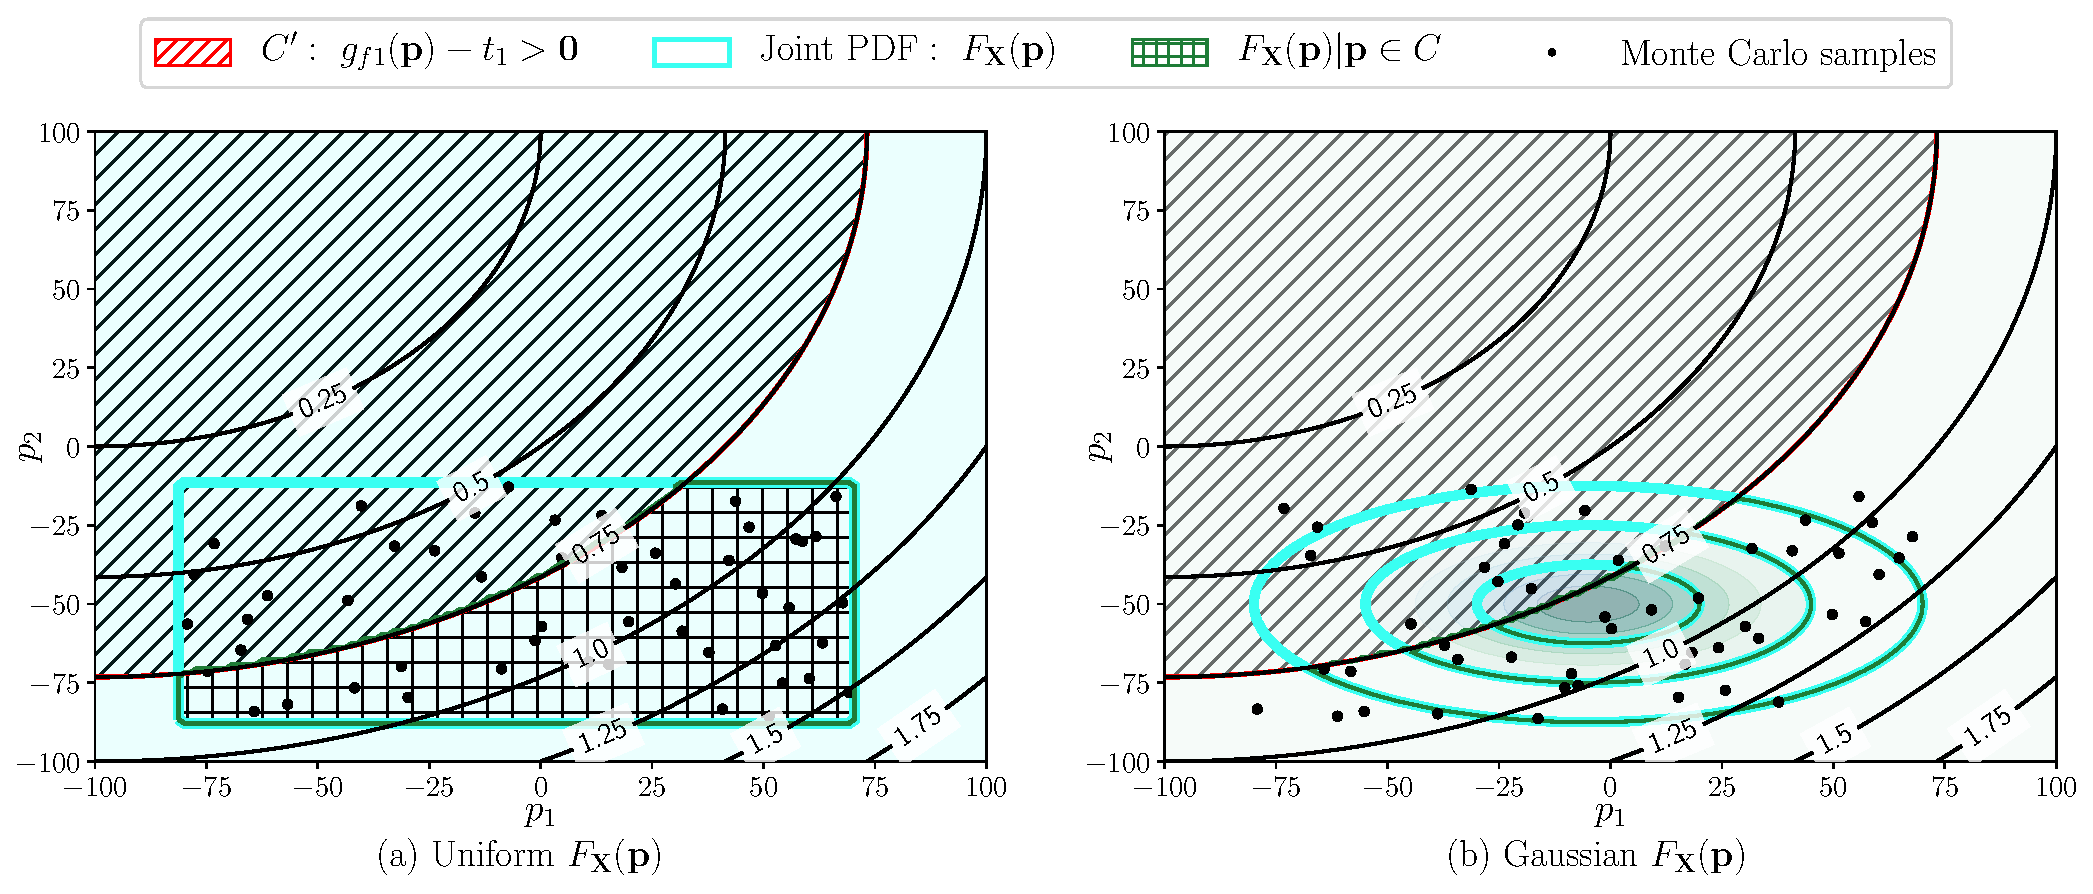
\includegraphics[width=0.9\textwidth]{1_2D_example_reliability.pdf}
	\caption{Contours of feasibility constraint $g_{f1}(\mathbf{p})$ in a 2D parameters space for different types of requirement \acp{PDF}}
	\label{fig:2Dexamplereliability}
\end{figure}

Only the Monte Carlo samples that lie within the set $C$ (shown as the unhatched region in Figure~\ref{fig:2Dexamplereliability}) are evaluated by $F_{\mathbf{X}}(\mathbf{p})$ and summed to compute the numerator of Equation~(\ref{eq:reliabilitymontecarlo}). All the Monte Carlo samples shown in Figure~\ref{fig:2Dexamplereliability} are evaluated by $F_{\mathbf{X}}(\mathbf{p})$ and summed to compute the denominator of Equation~(\ref{eq:reliabilitymontecarlo}). The reliability for the given requirement and capability can then be calculated as the quotient of the two sums.

We can now define buffer in the parameters space. Buffer is defined as the portion of the capability of a design reserved for changes in requirements \cite{Eckert2019}. In other words, the buffer set is defined as a set in the parameters space where sets $C$ and $R$ intersect.

\begin{equation} \label{eq:buffer}
	\textit{B} = \left\{\mathbf{p} \in \mathbb{R}^n~|~\mathbf{p} \in \left(C\cap R\right) \right\}.
\end{equation}

Excess is defined as the portion of the parameters space reserved for possible future changes in the requirements \cite{Eckert2019}. This is reflected by the set of parameter values that lie within the capability set $C$ but not within the requirement set $R$. 

\begin{equation} \label{eq:excess}
	\textit{E} = \left\{\mathbf{p} \in \mathbb{R}^n~|~\mathbf{p} \in \left(C\cap R'\right) \right\}.
\end{equation}

In other words, $B\cup E = C$.

The sets defined thus far are shown on the same 2-dimensional parameters space used for demonstrating the reliability calculation.

\begin{figure}[h!]
	\centering
	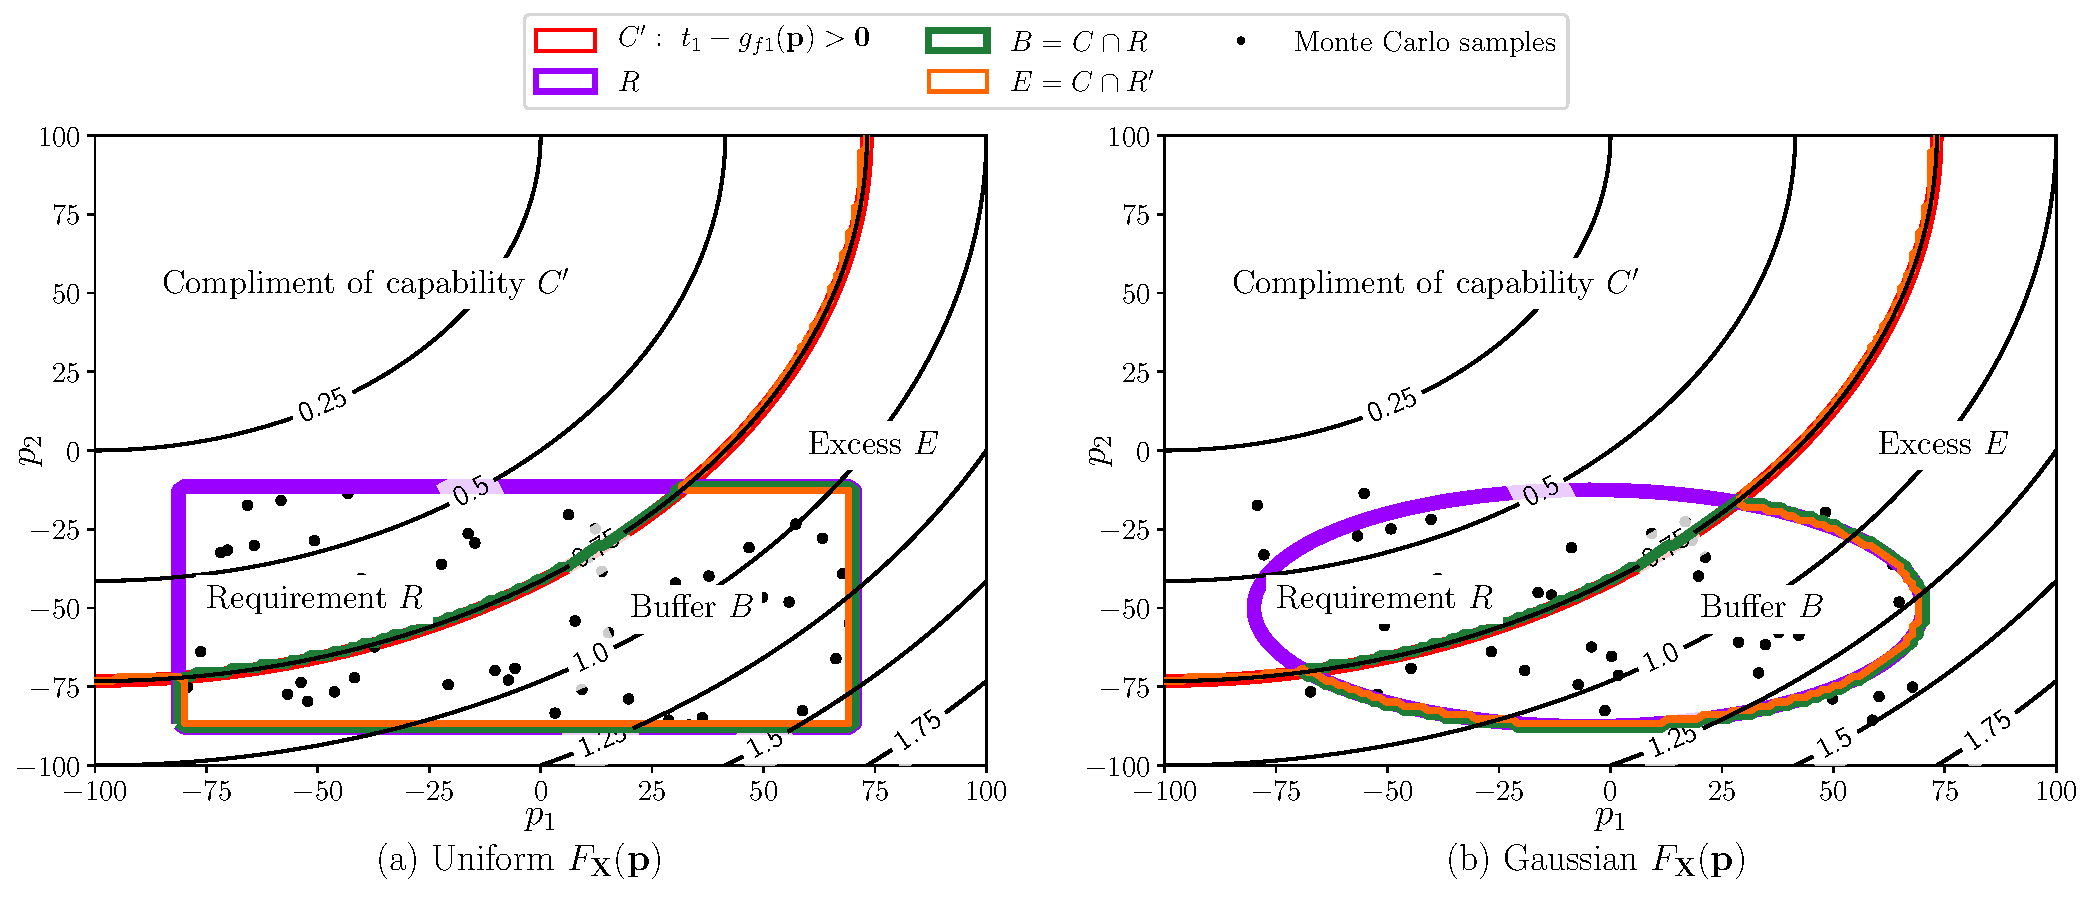
\includegraphics[width=0.9\textwidth]{2_2D_example_excess.pdf}
	\caption{Projections of the sets defining capability, requirements, buffer, and excess in a 2D parameters space for different types of requirement \acp{PDF}}
	\label{fig:2Dexampleexcess}
\end{figure}

We are particularly interested in minimizing excess during the product redesign cycle. We quantify excess using the volume of the set $E$ which can be found by Monte Carlo integration.

\begin{equation} \label{eq:excessmontecarlo}
	V_E \approx \dfrac{1}{N} {\sum\limits_{i=1}^{N} H\left(\mathbf{p}_i\right)}, ~\mathrm{where}~ H\left(\mathbf{p}_i\right)={\begin{cases}1&{\text{if }}\mathbf{p}_i\in E\\0&{\text{else}}\end{cases}},
\end{equation}

where $N$ is the number of samples from the parameters space used for the integration such that $\mathbf{p}_i \in \mathbb{R}^n$. However, a large number of Monte Carlo samples is needed to capture the complex profile of the set $E$ in multi-dimensional parameters spaces.

We can make use of the reliability $\mathbb{P}(\mathbf{p} \in C)$ calculation and the volume of the requirement set $R$ to indirectly estimate the volume of set $E$. The volume of $R$ can be computed analytically for a uniform or Gaussian distribution. For a uniform distribution, volume is given by the corresponding hyper-rectangle. For a Gaussian distribution, volume is given by the corresponding hyper-ellipsoid.

\begin{equation} \label{eq:Rmontecarlo}
	V_R = {\begin{cases} \prod\limits_{j=1}^{n} \left|b_j - a_j\right| &{\text{if }}F_\mathbf{X}(\mathbf{p})\text{ is uniform}\\\dfrac{\pi^2}{32}\prod\limits_{j=1}^{n} \left|b_j - a_j\right| &{\text{if }}F_\mathbf{X}(\mathbf{p})\text{ is Gaussian}\end{cases}}.
\end{equation}

We can compute the volume of set $C$ using the following approach.

\begin{equation} \label{eq:Cmontecarlo}
	V_C \approx \dfrac{1}{N} {\sum\limits_{i=1}^{N} H\left(\mathbf{p}_i\right)}, ~\mathrm{where}~ H\left(\mathbf{p}_i\right)={\begin{cases}1&{\text{if }}\mathbf{p}_i\in C\\0&{\text{else}}\end{cases}}.
\end{equation}

The reliability approximates the percentage of $R$ in $C$ and can be used as as proxy for the volume of $C\cap R$ such that $V_{C\cap R} \approx \mathbb{P}(\mathbf{p} \in C) \times V_R$. $V_E$ can now be approximated using

\begin{equation} \label{eq:excesssimple}
	V_E \approx V_C - \mathbb{P}(\mathbf{p} \in C) \times V_R.
\end{equation}

Having defined all the required design metrics, an optimization problem in terms of these metrics can be formulated such that excess is minimized while reliability constraints are met. We first define the context for the optimization problem in the form of an epoch-era analysis to simulate changing requirements throughout the product cycle.

%---------------------------------------------------------------------%
% Epoch era analysis
\subsection{Epoch era analysis for product redesign} \label{subsec:epochera}

We consider a problem where a product is redesigned as time progresses and the product advances through its development cycle or lifecycle. At the beginning of every epoch in the product cycle, the designer must choose a redesign choice from a list of available options. This list of options is given by the set of redesign choices defined as the set of non-negative integers $\mathcal{D} = \left\{0,1,2,\cdots,q\right\}$. Chaining multiple choices together results in a design arc defined as:

\begin{equation} \label{eq:designarc}
	\mathbf{D} = \left[D_1 ~ D_2 ~ \cdots ~ D_o\right]^{\mathrm{T}},
\end{equation}

with possible choices $D_d \in \mathcal{D}^o$, where $1 \leq o \leq q+1$. The maximum number of redesign choices $q + 1$ dictates the maximum number of possible design arc combinations where no choice is repeated twice. For example, consider a case where there are $q + 1 = 3$ redesign choices. We drop the transpose operator $^{\mathrm{T}}$ when reporting design arcs in this thesis for convenience. The possible design arcs that can be obtained for the set of redesign choices $\mathcal{D} = \left\{0,1,2\right\}$ is

\begin{equation*}
	\begin{aligned}
		& \mathbf{D}_1 = \left[0\right]\\
		& \mathbf{D}_2 = \left[0 ~ 1\right]\\
		& \mathbf{D}_3 = \left[0 ~ 1 ~ 2\right]\\
		& \mathbf{D}_4 = \left[0 ~ 2\right]\\
		& \mathbf{D}_5 = \left[0 ~ 2 ~ 1\right]\\
		& \mathbf{D}_6 = \left[1\right]\\
		& \mathbf{D}_7 = \left[1 ~ 0\right]\\
		& \mathbf{D}_8 = \left[1 ~ 0 ~ 2\right]\\
		& \mathbf{D}_9 = \left[1 ~ 2\right]\\
		& \mathbf{D}_{10} = \left[1 ~ 2 ~ 0\right]\\
		& \mathbf{D}_{11} = \left[2\right]\\
		& \mathbf{D}_{12} = \left[2 ~ 0\right]\\
		& \mathbf{D}_{13} = \left[2 ~ 0 ~ 1\right]\\
		& \mathbf{D}_{14} = \left[2 ~ 1\right]\\
		& \mathbf{D}_{15} = \left[2 ~ 1 ~ 0\right].\\
	\end{aligned}
\end{equation*}

These enumerations of the set $\mathcal{D}$ comprise a set of possible design arcs given by $\Omega_D$. The cardinality of $\Omega_D$ for a different number of redesign choices $q+1$ is given in Table~\ref{table:omegadcardinality}. For the previous example, the cardinality was $15$. The notation $|\Omega_D|$ is the cardinality operator applied to set $\Omega_D$.

\begin{table}[h!]
	\centering
	\renewcommand{\arraystretch}{1.0}% Wider
	\footnotesize\addtolength{\tabcolsep}{-5pt}
	\caption{Cardinality of set of possible design arcs $\mathbf{D}$}
	\label{table:omegadcardinality}
	\begin{tabular}{>{\centering\arraybackslash}p{2cm}>{\centering\arraybackslash}p{2cm}}
	\hline\hline
	\bf Number of redesign choices    & \bf Cardinality \\
	$q+1$ & $|\Omega_D|$ \\ \hline
	1  & 1 \\ 
	2 & 4 \\
	3 & 15 \\
	4 & 64 \\
	5 & 325 \\
	6 & 1956 \\
	\hline\hline
	\end{tabular}
\end{table}

We define a product cycle with $m$ number of epochs and $m$ number of corresponding decisions $S \in \mathcal{S}^m$, where $S_k$ is the decision for epoch $k$ and $\mathcal{S}$ is the set of possible decisions. In this chapter, we consider discrete redesign choices only. A non-negative integer value from the set $\mathcal{S}$ implies a redesign choice. A value of $-1$ implies no redesign is performed for the current epoch. This means that $\mathcal{S} = \left\{-1,0,1,2,\cdots,q\right\}$, where $q + 1$ is the number of available redesign choices.

The vector of all the decisions taken throughout the product cycle is referred to as the decision arc and is defined as

\begin{equation} \label{eq:decisionarc}
	\mathbf{S} = \left[S_1 ~ S_2 ~ \cdots ~ S_m\right]^{\mathrm{T}}.
\end{equation}

We also drop the transpose operator $^{\mathrm{T}}$ when reporting decision arcs in this thesis for convenience. The set of possible decision arcs that can be generated from the set of possible decisions $\mathcal{S}$ is governed by some feasibility constraints. A feasible decision arc cannot contain repeated choices in a manner similar to design arcs $\mathbf{D}$. For example, the decision arc $\mathbf{S} = \left[0 ~ -1 ~ 0 ~ -1 ~ 1 ~ 3\right]$ is infeasible since the choice $0$ was repeated twice, while the decision arc $\mathbf{S} = \left[0 ~ -1 ~ 2 ~ -1 ~ 1 ~ 3\right]$ is feasible since it has no repeated choices. Furthermore, the first decision cannot be empty, i.e. $S_1 \neq -1$. This is because a decision arc must begin with some sort of design. These restrictions make computing the cardinality of the set of possible decision arcs $\Omega_S$ challenging. However, the cardinality of $\Omega_S$ is given by a finite positive integer similar to $\Omega_D$ in Table~\ref{table:omegadcardinality}.

A corresponding design arc can be extracted from the decision arc by removing all negative components from $\mathbf{S}$ to obtain $\mathbf{D} = \left[0 ~ 2 ~ 1 ~ 3\right]$. 

For each epoch $k$, a design arc can be extracted by excluding values from $\mathbf{S}$ that are equal to $-1$. The vector $\mathbf{D}_k = \left[D_1 ~ D_2 ~ \cdots ~ D_o\right]$ represents this design arc for epoch $k$ where the components of $\mathbf{D}$ are non-negative integers and $o$ is the number of non-negative integers in $\mathbf{S}_k = \left[S_1 ~ S_2 ~ \cdots ~ S_k\right]$ for the current epoch $k$. For example, consider the following decision arc for a problem with $m=6$ epochs.

\begin{equation*} \label{eq:decisionarcex}
	\mathbf{S} = \left[0 ~ -1 ~ 2 ~ -1 ~ 1 ~ 3\right].
\end{equation*}

$m$ design arcs can be extracted from $\mathbf{S}$ for each epoch.

\begin{equation*}
	\begin{aligned}
		& \mathrm{epoch~} k=1: \mathbf{D}_1 = \left[0\right]\\
		& \mathrm{epoch~} k=2: \mathbf{D}_2 = \left[0\right]\\
		& \mathrm{epoch~} k=3: \mathbf{D}_3 = \left[0 ~ 2\right]\\
		& \mathrm{epoch~} k=4: \mathbf{D}_4 = \left[0 ~ 2\right]\\
		& \mathrm{epoch~} k=5: \mathbf{D}_5 = \left[0 ~ 2 ~ 1\right]\\
		& \mathrm{epoch~} k=6: \mathbf{D}_6 = \left[0 ~ 2 ~ 1 ~ 3\right].\\
	\end{aligned}
\end{equation*}

Logically, it follows that each design arc cannot feature repeated components due to the uniqueness of the positive decision arc components. Each design arc has a unique capability set $C_k$.

We now define the requirement arc as a vector of joint \acp{PDF} that has $m$ components. Each component corresponds to a different epoch $k$ with a requirement joint \ac{PDF} $F_{\mathbf{X}k}(\mathbf{p})$. The requirement arc is defined as

\begin{equation} \label{eq:requirementarc}
	\mathbf{R} = \left[F_{\mathbf{X}1}(\mathbf{p}) ~ F_{\mathbf{X}2}(\mathbf{p}) ~ \cdots ~ F_{\mathbf{X}m}(\mathbf{p})\right]^{\mathrm{T}}.
\end{equation}

The reliability for epoch $k$, $\mathbb{P}_k(\mathbf{p} \in C_k)$ can be calculated from $C_k$ (derived from $\mathbf{D}_k$) and the requirement joint \ac{PDF} $F_{\mathbf{X}k}(\mathbf{p})$ to yield a reliability vector defined as

\begin{equation} \label{eq:reliabilityvector}
	\mathbf{P}_{\mathbf{p} \in {C}} = \left[\mathbb{P}_1(\mathbf{p} \in C_1) ~ \mathbb{P}_2(\mathbf{p} \in C_2) ~ \cdots ~ \mathbb{P}_m(\mathbf{p} \in C_m)\right]^{\mathrm{T}}.
\end{equation}

For each epoch, a reliability threshold $P_k$ is defined to yield a vector of reliability thresholds defined as

\begin{equation} \label{eq:reliabilitythvector}
	\mathbf{P}_{th} = \left[P_1 ~ P_2 ~ \cdots ~ P_m\right]^{\mathrm{T}}.
\end{equation}

The volume of the excess set for epoch $k$, $V_{Ek}$ can be calculated from $C_k$ and the requirement joint \ac{PDF} $F_{\mathbf{X}k}(\mathbf{p})$ using Equations~(\ref{eq:excess}) and (\ref{eq:excesssimple}) to yield an excess vector defined as

\begin{equation} \label{eq:excessvector}
	\mathbf{E} = \left[V_{E1} ~ V_{E2} ~ \cdots ~ V_{Em}\right]^{\mathrm{T}}.
\end{equation}

The cumulative excess for a given decision arc can be formulated as

\begin{equation} \label{eq:excesscumulative}
	E_c = \sum\limits_{k=1}^{m} V_{Ek}.
\end{equation}

In addition to the decision arc $\mathbf{S}$, a fixed design concept $c_t\in\mathcal{C}$ is defined. The concept type $c_t$ is selected at the very beginning of the epoch-era analysis and does not change throughout epochs. The choice of $c_t$ dictates the list of redesign choices available for the remainder of the product cycle. $\mathcal{C}$ is the set of concept choices whose elements are all non-negative integers. This means that $\mathcal{C} = \left\{0,1,2,\cdots,r\right\}$, where $r + 1$ is the number of available concept choices.

Each concept type $c_t$ has a set of redesign options $\mathcal{D}_t$ with $q+1$ redesign choices attached to it. Accordingly, each concept type $c_t$ will have a set of possible design arcs $\Omega_{Dt}$ and a set of possible decision arcs $\Omega_{St}$. The combination of a concept and design arc $\left\{c,\mathbf{D}\right\}$ will be referred to as a design arc in this thesis for conciseness. Similarly, the combination of a concept and a decision arc $\left\{c,\mathbf{S}\right\}$ will be referred to as a decision arc.

The cardinality of the set of possible design arcs $\Omega_{cD}$ is simply obtained by adding up all the cardinalities of the sets $\Omega_{Dt}$ for a given set of concept choices $\mathcal{C}$

\begin{equation} \label{eq:cardinailitycdarc}
	\beta = |\Omega_{cD}| = \sum\limits_{t=0}^{r} |\Omega_{Dt}|,
\end{equation}

where $|\Omega_{Dt}|$ can be obtained from Table~\ref{table:omegadcardinality} knowing the number of redesign choices $q+1$ for each concept. The set of possible design arcs represents the feasible design space in this chapter and is defined as

\begin{equation} \label{eq:feasibledesignset}
	\Omega_{cD} = \left\{\left\{c,\mathbf{D}\right\}_1,\left\{c,\mathbf{D}\right\}_2,\cdots,\left\{c,\mathbf{D}\right\}_\beta\right\}.
\end{equation}

A similar approach can be used to calculate the cardinality of the set of possible decision arcs $\Omega_{cS}$ although we do not need to compute it in this chapter.

\begin{equation} \label{eq:cardinailitycsarc}
	|\Omega_{cS}| = \sum\limits_{t=0}^{r} |\Omega_{St}|.
\end{equation}

We now formulate an optimization problem for choosing the optimal concept $c$ and decision arc $\mathbf{S}$ such that cumulative excess $E_c$ is minimized subject to reliability constraints $\mathbf{g}(c,\mathbf{S}) = \mathbf{P}_{th} - \mathbf{P}_{\mathbf{p} \in \mathbf{C}} \le \mathbf{0}$

\begin{equation}
	\label{eq:TSEoptproblem}
	\begin{aligned}
		& \underset{\{c,\mathbf{S}\}\in\Omega_{cS}}{\text{minimize}}
		& & {f}(c,\mathbf{S};\mathbf{R}) = E_c = \sum\limits_{k=1}^{m} V_{Ek}(c,\mathbf{D}_k;F_{\mathbf{X}k}(\mathbf{p}))\\
		& \text{subject to}
		& & \mathbf{g}(c,\mathbf{S};\mathbf{R}) = \mathbf{P}_{th} - \mathbf{P}_{\mathbf{p} \in \mathbf{C}} \le \mathbf{0}\\
		& \text{where,}
		& & \Omega_{cS}\text{: all feasible decision arcs}.\\
	\end{aligned}
\end{equation}

We also define a second optimization problem to simulate the effect of accumulating costs that can be incurred throughout a product's lifecycle. Since we focus on aerospace applications in this chapter, we consider the cumulative weight of the decision arc to be a reflection of cumulative costs such as fuel \cite{Thomsen2016}.

\begin{equation}
	\label{eq:optproblemweight}
	\begin{aligned}
		& \underset{\{c,\mathbf{S}\}\in\Omega_{cS}}{\text{minimize}}
		& & {f}(c,\mathbf{S}) = W_c = \sum\limits_{k=1}^{m} W_{k}(c,\mathbf{D}_k)\\
		& \text{subject to}
		& & \mathbf{g}(c,\mathbf{S};\mathbf{R}) = \mathbf{P}_{th} - \mathbf{P}_{\mathbf{p} \in \mathbf{C}} \le \mathbf{0}\\
		& \text{where,}
		& & \Omega_{cS}\text{: all feasible decision arcs}.\\
	\end{aligned}
\end{equation}

The problems in Equations~(\ref{eq:TSEoptproblem}) and (\ref{eq:optproblemweight}) are solved using a combinatorial optimization algorithm rather than a discrete optimization algorithm. This is because the feasible set $\Omega_{cS}$ is not given by the possible combinations of integers in $\mathcal{S} = \left\{-1,0,1,2,\cdots,q\right\}$. The choice of concept is restricted to non-negative integers, while the decision arc may not feature repeated non-negative integers as explained earlier. As a result, the set $\Omega_{cS}$ must be algorithmically defined as is done with combinatorial optimization problems such as simulated annealing \cite{Kirkpatrick1983}. However, such heuristic optimization algorithms require a large number of iterations to converge making computations intractable especially when reliability constraints are involved. A mixed variable optimization variant of \ac{MADS} is provided by the \texttt{NOMAD} algorithm \cite{Abramson2009}. This implementation of \ac{MADS} allow users to specify categorical constraints via an extended poll subroutine and is called during the search step \cite{Abramson2004,Abramson2008}.

The optimization problems given by Equations~(\ref{eq:TSEoptproblem}) and (\ref{eq:optproblemweight}) yield a solution $\mathbf{x}^*(\mathbf{R})$ which depends on the requirement arc $\mathbf{R}$. The nature of requirements is that they are subject to change. As a result, we adopt a set-based design strategy to manage changing requirements.

%---------------------------------------------------------------------%
% Set-based approach
\subsection{Set-based design for uncertain requirements} \label{subsec:SBDproblem}

%f: objective functions
%g: constraint functions
%n: dimensionality of parameters space
%i: requirement set sample index 
%j: component index of bounds vectors for Gaussian and uniform pdfs
%m: number of stages
%k: index of stage
%o: number of designs in design arcs
%d: index of design decision in design arc
%q: number of redesign (deposit) choices
%r: number of concept choices
%s: number of SBD requirement arc samples (cardinality)
%w: index of requirement arc sample
%v: number of choices for joint PDF
%t: type of PDF set
%e: number of linear interpolation samples for generating R_v
%\alpha: number of designs for cut-off
%\beta: number of possible concept/design arcs
%\lambda: index of concept/design arcs
%\zeta: number of possible enumerations of decision arcs from design arcs
%\gamma: index of decision arc in enumerations from design arcs

The set-based design strategy involves sampling requirement arcs $\mathbf{R}$ from the set of possible requirement arcs $\Omega_R$. A sample from the set $\Omega_R$, $\mathbf{R}_w$ involves populating the requirement arc with joint \acp{PDF} for each epoch $k$ by selecting a joint \ac{PDF} from the set of possible joint \acp{PDF} $\mathcal{R} = \left\{F_{\mathbf{X}1}(\mathbf{p}),F_{\mathbf{X}2}(\mathbf{p}),\cdots,F_{\mathbf{X}v}(\mathbf{p})\right\}$, where $v$ is the number of joint \ac{PDF} choices. $\mathbf{R}_w$ is constructed by selecting $m$ joint \acp{PDF} from $\mathcal{R}$ such that $\mathbf{R}_w \in \mathcal{R}^m$. $\Omega_R$ is defined as

\begin{equation} \label{eq:Rarcsample}
	\Omega_R = \left\{\mathbf{R}_1,\mathbf{R}_2\cdots,\mathbf{R}_s\right\},
\end{equation}

where $s = |\Omega_R|$ is the cardinality of $\Omega_R$.

The set of joint \ac{PDF} choices $\mathcal{R}$ is constructed by generating different joint \acp{PDF} defined by their mean vector $\boldsymbol{\mu}$, interval vector $\boldsymbol{\sigma}$, and type $t\in\mathcal{T} = \left\{\mathrm{``Uniform"},\mathrm{``Gaussian"}\right\}$. The interval vector $\boldsymbol{\sigma}$ is the same as the standard deviation vector defined for the Gaussian joint \ac{PDF} in Equation~(\ref{eq:gaussianpdf}). For a uniform joint \ac{PDF}, the bounds are obtained from the interval vector such that $\mathbf{a} = \boldsymbol{\mu} - 3\boldsymbol{\sigma}$ and $\mathbf{b} = \boldsymbol{\mu} + 3\boldsymbol{\sigma}$. This allows any joint \ac{PDF} to be fully parametrized by three parameters, the type $t$, the mean vector $\boldsymbol{\mu}$, and the interval vector $\boldsymbol{\sigma}$.

The method for populating the set $\mathcal{R}$ is based on the designer's experience with the requirements and previous knowledge. For example if requirements are expected to become well-defined over time around a certain value in the parameters space, then a matrix of mean vectors $\mathbf{M} = \left[\boldsymbol{\mu}_1,\boldsymbol{\mu}_2,\cdots,\boldsymbol{\mu}_e\right]^{\textrm{T}}$ and a matrix of interval vectors $\boldsymbol{\Sigma} = \left[\boldsymbol{\sigma}_1,\boldsymbol{\sigma}_2,\cdots,\boldsymbol{\sigma}_e\right]^{\textrm{T}}$ can be obtained by linearly interpolating between the start and end states given by $\boldsymbol{\mu}_1,\boldsymbol{\sigma}_1$ and $\boldsymbol{\mu}_e,\boldsymbol{\sigma}_e$, respectively for each type of joint \ac{PDF}. 

An example of this kind of interpolation search strategy is shown in Figure~\ref{fig:2Dexampleinterp} for the same 2D example used in Section~\ref{subsec:designmetrics}.

\begin{figure}[h!]
	\centering
	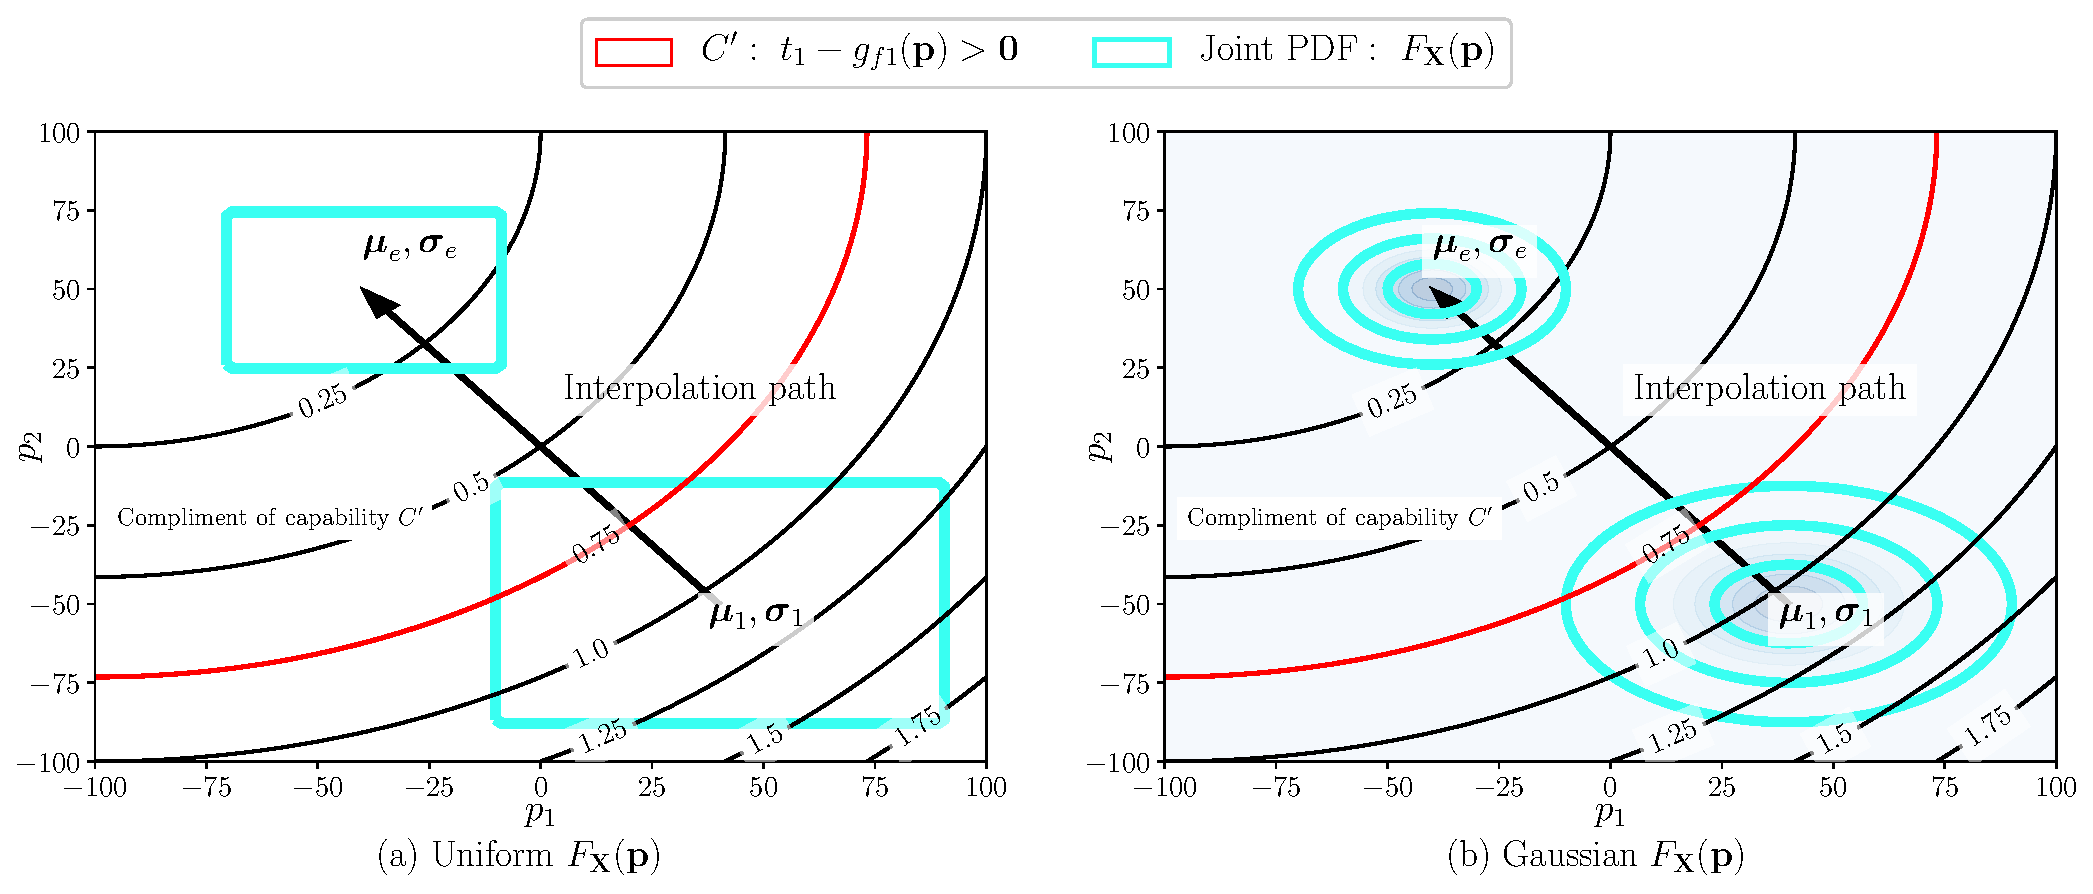
\includegraphics[width=0.9\textwidth]{3_2D_example_interpolation.pdf}
	\caption{Interpolation between two end states of different joint \acp{PDF} in a 2D parameters space}
	\label{fig:2Dexampleinterp}
\end{figure}

The set of possible requirement arcs $\Omega_R$ spans every possible combination of the joint \ac{PDF} types $t$, means $\mathbf{M}$, and intervals $\boldsymbol{\Sigma}$. Consider an example with $m=6$ epochs. If $e=5$ interpolation levels are used to obtain $\mathbf{M}$ and $\boldsymbol{\Sigma}$ and two \ac{PDF} types 

\begin{equation*}
	\mathcal{T} = \left\{\mathrm{``Uniform"},\mathrm{``Gaussian"}\right\}
\end{equation*} 

are available, the number of choices $v$ for $\mathcal{R}$ and the cardinality $s$ for $\Omega_R$ is calculated as

\begin{equation*}
	\begin{aligned}
		& v = e \times e \times |\mathcal{T}| = 5 \times 5 \times 2 = 50,~\textrm{and}\\
		& s = |\Omega_R| = m^v = 6^{50},~\mathrm{respectively}.\\
	\end{aligned}
\end{equation*}

It can be deduced that a small increase in the number of joint \ac{PDF} choices causes the cardinality of $\Omega_R$ to increase exponentially. For practicality, only the first few elements of $\Omega_R$ will be used during the set-based design analysis and $s$ will be capped at $10^5$ samples. The reasons for this choice will be explained in results Section~\ref{sec:TSEresults}.

The first set-based solution is obtained by solving the optimization problem in Equation~(\ref{eq:TSEoptproblem}) for every requirement arc sample $\mathbf{R}_w$ in $\Omega_R$ to obtain a corresponding solution $\mathbf{x}_S^*(\mathbf{R}_w) = \left\{c^*,\mathbf{S}^*\right\}(\mathbf{R}_w)$. In order to compare the overdesign levels across different design arcs rather than different decision arcs, the corresponding optimal design arc $\mathbf{D}^*$ can be extracted from the optimal decision arc $\mathbf{S}^*$ to obtain the solution $\mathbf{x}^*(\mathbf{R}_w) = \left\{c^*,\mathbf{D}^*\right\}(\mathbf{R}_w)$

The set of parametric optimal design arcs with respect to excess is defined as

\begin{equation} \label{eq:SBDexcessopt}
	S_E^* = \left\{\mathbf{x}^*(\mathbf{R}_1),\mathbf{x}^*(\mathbf{R}_2)\cdots,\mathbf{x}^*(\mathbf{R}_s)\right\}.
\end{equation}

We track the number of times a specific design arc $\left\{c,\mathbf{D}\right\}_\lambda$ appears as the solution to the parametric optimization problem in $S_E^*$ via a design optimality vector defined as

\begin{equation} \label{eq:optimalityvec}
	\mathbf{N}_E = \left[n_{E1} ~ n_{E2} ~ \cdots ~ n_{E\beta}\right]^{\mathrm{T}},
\end{equation}

where $n_{E\lambda}$ is equal to the number of times design arc $\left\{c,\mathbf{D}\right\}_\lambda \in \Omega_{cD}$ is repeated in $S_E^*$ and gives the frequency of each design arc. The top $\alpha$ design arcs with the largest $n_{E\lambda}$ values are selected as the set-based solution representing the best performing design arcs in terms of minimizing over-design.

\begin{equation} \label{eq:SBDexcess}
	S_E = \left\{\left\{c,\mathbf{D}\right\}_{E1},\left\{c,\mathbf{D}\right\}_{E2}\cdots,\left\{c,\mathbf{D}\right\}_{E\alpha}\right\},
\end{equation}

where the subscript $E1,E2,\cdots,E\alpha$ indicates that the corresponding base is ordered by frequency in the set of parametric optimal solutions with respect to excess $S_E^*$.

The same procedure is repeated for the optimization problem in Equation~(\ref{eq:optproblemweight}) to obtain the second set-based solution comprising the best performing design arcs in terms of minimizing weight throughout the product cycle.

\begin{equation} \label{eq:SBDweight}
	S_W = \left\{\left\{c,\mathbf{D}\right\}_{W1},\left\{c,\mathbf{D}\right\}_{W2}\cdots,\left\{c,\mathbf{D}\right\}_{W\alpha}\right\},
\end{equation}

where the subscripts $W1,W2,\cdots,W\beta$ indicate that the corresponding base is ordered by frequency in the set of parametric optimal solutions with respect to weight $S_W^*$.

Algorithm~\ref{algo:SBDOptalgo} describes the methodology to be followed for obtaining the set of optimal design arcs with respect to excess or weight.

\begin{algorithm}
	\DontPrintSemicolon % Some LaTeX compilers require you to use \dontprintsemicolon instead
	\KwIn{
		Set of possible requirement arcs $\Omega_R$, Set of possible design arcs $\Omega_{cD}$
	}
	\KwOut{$S_{E}$}
	Initialize design optimality vector $\mathbf{N}_E = \left[n_{E1},n_{E2},\cdots,n_{E\beta}\right] = \mathbf{0}$\;	
	\For{$w \gets 1$ to $s$} {
		Solve the parametric optimization problem in Equation~(\ref{eq:TSEoptproblem}) to obtain optimal decision arc $\mathbf{x}_S^*(\mathbf{R}_w) = \left\{c^*,\mathbf{S}^*\right\}(\mathbf{R}_w)$\;
		Reduce optimal decision arc to optimal design arc by eliminating $-1$ components of $\mathbf{S}^*$ to obtain $\mathbf{x}^*(\mathbf{R}_w) = \left\{c^*,\mathbf{D}^*\right\}(\mathbf{R}_w)$\;
		Augment $S_{E}^* \gets S_{E}^* \cup \{ \mathbf{x}^*(\mathbf{R}_w) \} $\;
		Find $\lambda$ corresponding to $\left\{c^*,\mathbf{D}^*\right\}$\;
		Award design arc $n_{E\lambda} \gets n_{E\lambda} + 1$\;
	}
	Sort design optimality vector $\mathbf{N}_E$ in descending order\;
	Select top $\alpha$ design arcs with largest values $n_{E\lambda}$ to obtain set of optimal design arcs $S_E = \left\{\left\{c,\mathbf{D}\right\}_{E1},\left\{c,\mathbf{D}\right\}_{E2}\cdots,\left\{c,\mathbf{D}\right\}_{E\alpha}\right\}$\;
	\caption{Pseudo-algorithm for obtaining the set of optimal design arcs $S_{E}$}
	\label{algo:SBDOptalgo}
\end{algorithm}

The third set-based solution is the robust design set. We define robustness of a design arc by the number of requirement arcs satisfied from the set $\Omega_R$. We evaluate the feasibility of each design arc $\left\{c,\mathbf{D}\right\}_\lambda$ sampled from the set of possible design arcs in Equation~(\ref{eq:feasibledesignset}) with respect to every requirement arc $\mathbf{R}_w$ in $\Omega_R$.

We generate all the possible decision arcs for a given design arc $\left\{c,\mathbf{D}\right\}_\lambda$. These combinations are generated by randomly inserting the $-1$ decisions into the design arc vector until it has as many components as there are epochs $m$. We show this using an example. Consider the design arc $\left\{c = 1,\mathbf{D} = \left[2 ~ 0 ~ 1\right]\right\}$. The possible decision arcs are

\begin{equation*}
	\begin{aligned}
		& \left\{c = 1,\mathbf{S} = \left[2 ~ -1 ~ -1 ~ -1 ~ 0 ~ 1\right]\right\}\\
		& \left\{c = 1,\mathbf{S} = \left[2 ~ -1 ~ -1 ~ 0 ~ -1 ~ 1\right]\right\}\\
		& \left\{c = 1,\mathbf{S} = \left[2 ~ -1 ~ -1 ~ 0 ~ 1 ~ -1\right]\right\}\\
		& \left\{c = 1,\mathbf{S} = \left[2 ~ -1 ~ 0 ~ -1 ~ 1 ~ -1\right]\right\}\\
		& \left\{c = 1,\mathbf{S} = \left[2 ~ -1 ~ 0 ~ 1 ~ -1 ~ -1\right]\right\}\\
		& \left\{c = 1,\mathbf{S} = \left[2 ~ 0 ~ -1 ~ 1 ~ -1 ~ -1\right]\right\}\\
		& \left\{c = 1,\mathbf{S} = \left[2 ~ 0 ~ 1 ~ -1 ~ -1 ~ -1\right]\right\}.\\
	\end{aligned}
\end{equation*}

These enumerations result in a set of the decision arcs defined as

\begin{equation} \label{eq:enumeratedcS}
	S_{cD} = \left\{\left\{c,\mathbf{S}\right\}_{1},\left\{c,\mathbf{S}\right\}_{2}\cdots,\left\{c,\mathbf{S}\right\}_{\zeta}\right\},\mathrm{~where~} \left\{c,\mathbf{S}\right\}_{\gamma} \in S_{cD}
\end{equation}

and $\zeta$ is the number of possible enumerations. In the previous example $\zeta = 7$.

The feasibility in terms of reliability is checked for every enumerated decision arc $\left\{c,\mathbf{S}\right\}_{\gamma}$ for a given $\left\{c,\mathbf{D}\right\}_\lambda$ and requirement arc $\mathbf{R}_w$ using $\mathbf{g}(c_{\gamma},\mathbf{S}_{\gamma};\mathbf{R}_w) = \mathbf{P}_{th} - \mathbf{P}_{\mathbf{p} \in \mathbf{C}} \le \mathbf{0}$. If any of the decision arcs in set $S_{cD}$ satisfy all the reliability constraints then the corresponding design arc $\left\{c,\mathbf{D}\right\}_\lambda$ is considered feasible. We track the number of requirement arcs satisfied by design arc $\left\{c,\mathbf{D}\right\}_\lambda$ through a robustness vector defined as

\begin{equation} \label{eq:robustnessvec}
	\mathbf{N}_R = \left[n_{R1} ~ n_{R2} ~ \cdots ~ n_{R\beta}\right]^{\mathrm{T}},
\end{equation}

where $n_{R\lambda}$ is equal to the number of requirement arcs $\mathbf{R}_w \in \Omega_R$ satisfied by design arc $\left\{c,\mathbf{D}\right\}_\lambda \in \Omega_{cD}$. The top $\alpha$ design arcs with the largest $n_{R\lambda}$ values are considered as the robust design set.

\begin{equation} \label{eq:SBDrobust}
	S_R = \left\{\left\{c,\mathbf{D}\right\}_{R1},\left\{c,\mathbf{D}\right\}_{R2}\cdots,\left\{c,\mathbf{D}\right\}_{R\alpha}\right\},
\end{equation}

where the subscripts $R1,R2,\cdots,R\alpha$ indicate that these design arcs are ordered by number of requirement arcs satisfied from the set $\Omega_R$.

The final set-based solution is the flexible design set. All the possible design arcs form the set $\Omega_{cD}$ are ranked in terms of filtered outdegree. The filtered outdegree is defined as the number of possible design arcs that can be obtained from the current design arc by adding exactly one redesign choice that is not a component of the current design arc. The filtered outdegree for a design arc $\left\{c,\mathbf{D}\right\}_\lambda$ having $o$ components and $q + 1$ redesign choices is simply equal to

\begin{equation} \label{eq:filteredoutdegree}
	FO_{\lambda} = q - o.
\end{equation}

The top $\alpha$ design arcs in terms of filtered outdegree are considered as the flexible design set.

\begin{equation} \label{eq:SBDflexible}
	S_F = \left\{\left\{c,\mathbf{D}\right\}_{F1},\left\{c,\mathbf{D}\right\}_{F2}\cdots,\left\{c,\mathbf{D}\right\}_{F\alpha}\right\},
\end{equation}

where the subscript $F1,F2,\cdots,F\alpha$ indicate that these design arcs are ordered by filtered outdegree $FO$.

Algorithm~\ref{algo:SBDRobustalgo} describes the methodology to be followed for obtaining the sets of robust and flexible design arcs.

\begin{algorithm}
	\DontPrintSemicolon % Some LaTeX compilers require you to use \dontprintsemicolon instead
	\KwIn{
		Set of possible requirement arcs $\Omega_R$, Set of possible design arcs $\Omega_{cD}$
	}
	\KwOut{$S_{R}$, $S_{F}$}
	Initialize design robustness vector $\mathbf{N}_R = \left[n_{R1},n_{R2},\cdots,n_{R\beta}\right] = \mathbf{0}$\;	
	\For{$\lambda \gets 1$ to $\beta$} {
		Enumerate possible decision arcs from $\left\{c,\mathbf{D}\right\}_\lambda$ to obtain the set $S_{cD} = \left\{\left\{c,\mathbf{S}\right\}_{1},\left\{c,\mathbf{S}\right\}_{2}\cdots,\left\{c,\mathbf{S}\right\}_{\zeta}\right\}$\;
		\For{$w \gets 1$ to $s$} {
			\For{$\gamma \gets 1$ to $\zeta$} {
				
				\If{$\mathbf{g}(c_{\gamma},\mathbf{S}_{\gamma};\mathbf{R}_w) \le \mathbf{0}$} {
					Award design arc $n_{R\lambda} \gets n_{R\lambda} + 1$\;
					\textbf{break}
				}
			
			}
		}
		Compute filtered outdegree for $\left\{c,\mathbf{D}\right\}_\lambda$ using $FO_{\lambda} = q - o$\;
		Augment design flexibility vector $\mathbf{N}_F \gets \mathbf{N}_F \cup \{ FO_{\lambda} \} $\;
	}
	Sort design robustness vector $\mathbf{N}_R$ in descending order\;
	Select top $\alpha$ design arcs with largest values $n_{R\lambda}$ to obtain set of robust design arcs $S_R = \left\{\left\{c,\mathbf{D}\right\}_{R1},\left\{c,\mathbf{D}\right\}_{R2}\cdots,\left\{c,\mathbf{D}\right\}_{R\alpha}\right\}$\;
	Sort design flexibility vector $\mathbf{N}_F$ in descending order\;
	Select top $\alpha$ design arcs with largest values $FO_{\lambda}$ to obtain set of flexible design arcs $S_F = \left\{\left\{c,\mathbf{D}\right\}_{F1},\left\{c,\mathbf{D}\right\}_{F2}\cdots,\left\{c,\mathbf{D}\right\}_{F\alpha}\right\}$\;
	\caption{Pseudo-algorithm for obtaining the sets of robust $S_{R}$ and flexible $S_{F}$ design arcs}
	\label{algo:SBDRobustalgo}
\end{algorithm}

We summarize the procedure for obtaining the set-based solutions $S_E,S_W,S_R$, and $S_F$ in Figure~\ref{fig:methodology}.

\begin{figure}[h!]
	\centering
	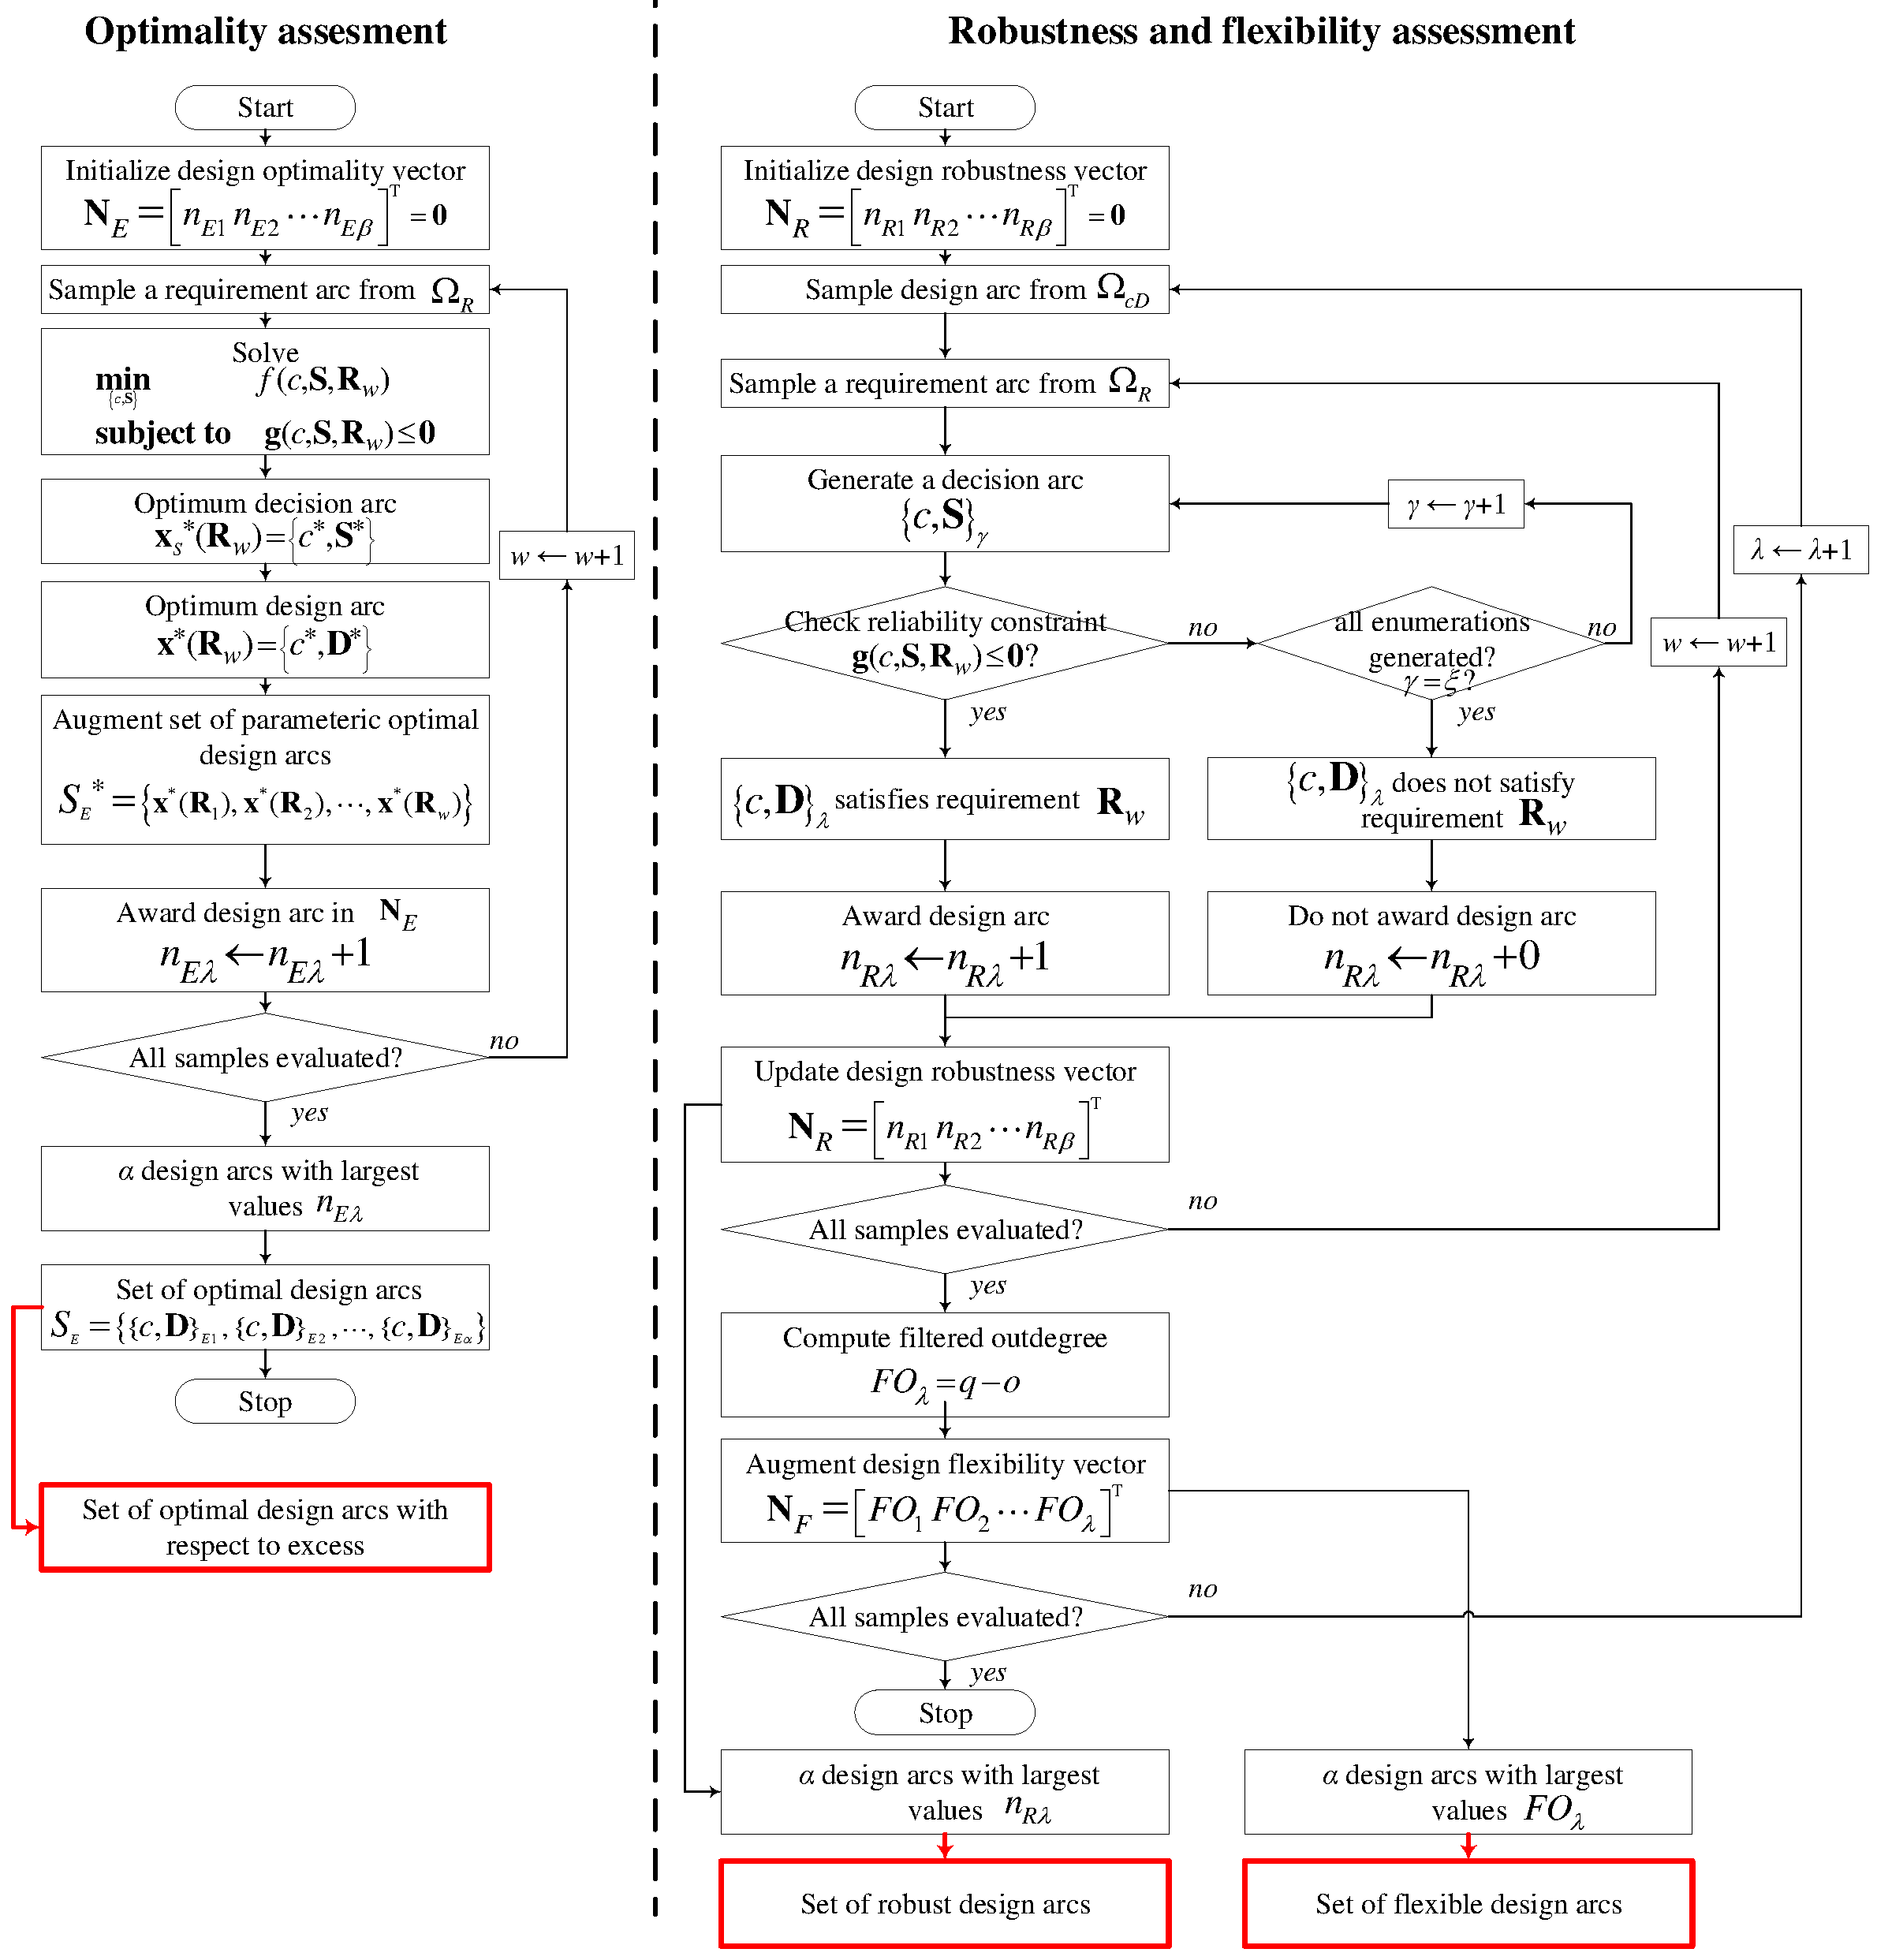
\includegraphics[width=0.99\textwidth]{4_methodology_V2.pdf}
	\caption{Summary of methodology for generating set-based solutions}
	\label{fig:methodology}
\end{figure}

A tradespace is used to visualize these solution sets for comparison.

%---------------------------------------------------------------------%
% Tradespace exploration
\subsection{Tradespace exploration for comparing solution sets} \label{subsec:TSE}

A tradespace is constructed by plotting the volume of the capability set $C$, given by $V_c$, against the weight of each design arc. The volume of capability set $C$ is chosen as the utility since it is independent of the requirement joint \ac{PDF}. This allows for a fair comparison between different design arcs. The weight is chosen as the cost metric for the tradespace.

The volume of the capability set $V_c$ is plotted against weight $W$ for every possible design arc in the set $\Omega_{cD}$ to show the feasible design set.

The design arcs in sets $S_E,S_W,S_R$, and $S_F$ are also projected on the same tradespace to compare their relative positions and sizes.

The Pareto front for such a tradespace can be obtained by solving the following biobjective problem:

\begin{equation}
	\label{eq:optproblembiobj}
	\begin{aligned}
		& \underset{\{c,\mathbf{D}\}\in\Omega_{cD}}{\text{minimize}}
		& & {f_1}(c,\mathbf{D}) = -V_c(c,\mathbf{D})\\
		& & & {f_2}(c,\mathbf{D}) = \textrm{W}\left(c,\mathbf{D}\right).\\
	\end{aligned}
\end{equation}

The positioning of sets $S_E,S_W,S_R$, and $S_F$ relative to the Pareto set obtained by solving the problem in Equation~(\ref{eq:optproblembiobj}) provides a measure for the dominance of each design set.

We will apply the methodology developed in this section to a remanufacturing design problem of a \ac{TRS}.

%========================= APPLICATION PROBLEM =======================%
\section{Application problem} \label{sec:TSEcasestudy}

We demonstrate the importance of minimizing excess in aerospace structural design by applying our methodology to the design of a \acf{TRS}. The \ac{TRS} is remanufactured by \ac{AM} techniques to increase the stiffness of the outer casing in response to changing requirements for the temperature loads. The \ac{TRS} can undergo multiple redesigns as given by a decision arc during its product cycle. We begin by describing the available stiffener designs and the thermomechanical models associated with them.

%---------------------------------------------------------------------%
% Stiffener and thermomechanical model
\subsection{Stiffener deposition on \ac{TRS} outercasing} \label{subsec:stiffeners}

Stiffeners deposited on the outer casing of the \ac{TRS} involve the application of heat to the outer casing (the substrate) to deposit material on its surface. The application of large heat fluxes to the surface of a structure causes residual distortion that persists after the removal of the heat source. This residual distortion affects the structural performance of the structure when loads are applied during operation. As a result, the residual stresses experienced by the \ac{TRS} due to deposition of a stiffener must be quantified prior to any structural analysis.

The residual stress tensors that persist after removal of the equivalent heat flux are stored and applied during the analysis of the thermal load case.

There are several stiffener geometries available to the designer of the \ac{TRS} given by the set of possible design arcs $\Omega_{cD}$. We draw inspiration from commonly used standard stiffener designs to generate concepts and design choices \cite{USArmyMaterielCommand1970}. The design space consists of three possible deposition concepts $\mathcal{C} = \left\{0,1,2\right\}$. Concept $c=0$ is a "wavy" stiffener that has three redesign choices $\mathcal{D}_0 = \left\{0,1,2\right\}$. Concept $c=1$ is a "hatched" stiffener that has five redesign choices $\mathcal{D}_1 = \left\{0,1,2,3,4\right\}$. Concept $c=2$ is a "tubular" stiffener that has four redesign choices $\mathcal{D}_2 = \left\{0,1,2,3\right\}$. We illustrate these concepts and their respective design choices in Figure~\ref{fig:designspacestiff}.

\begin{figure}[h!]
	\centering
	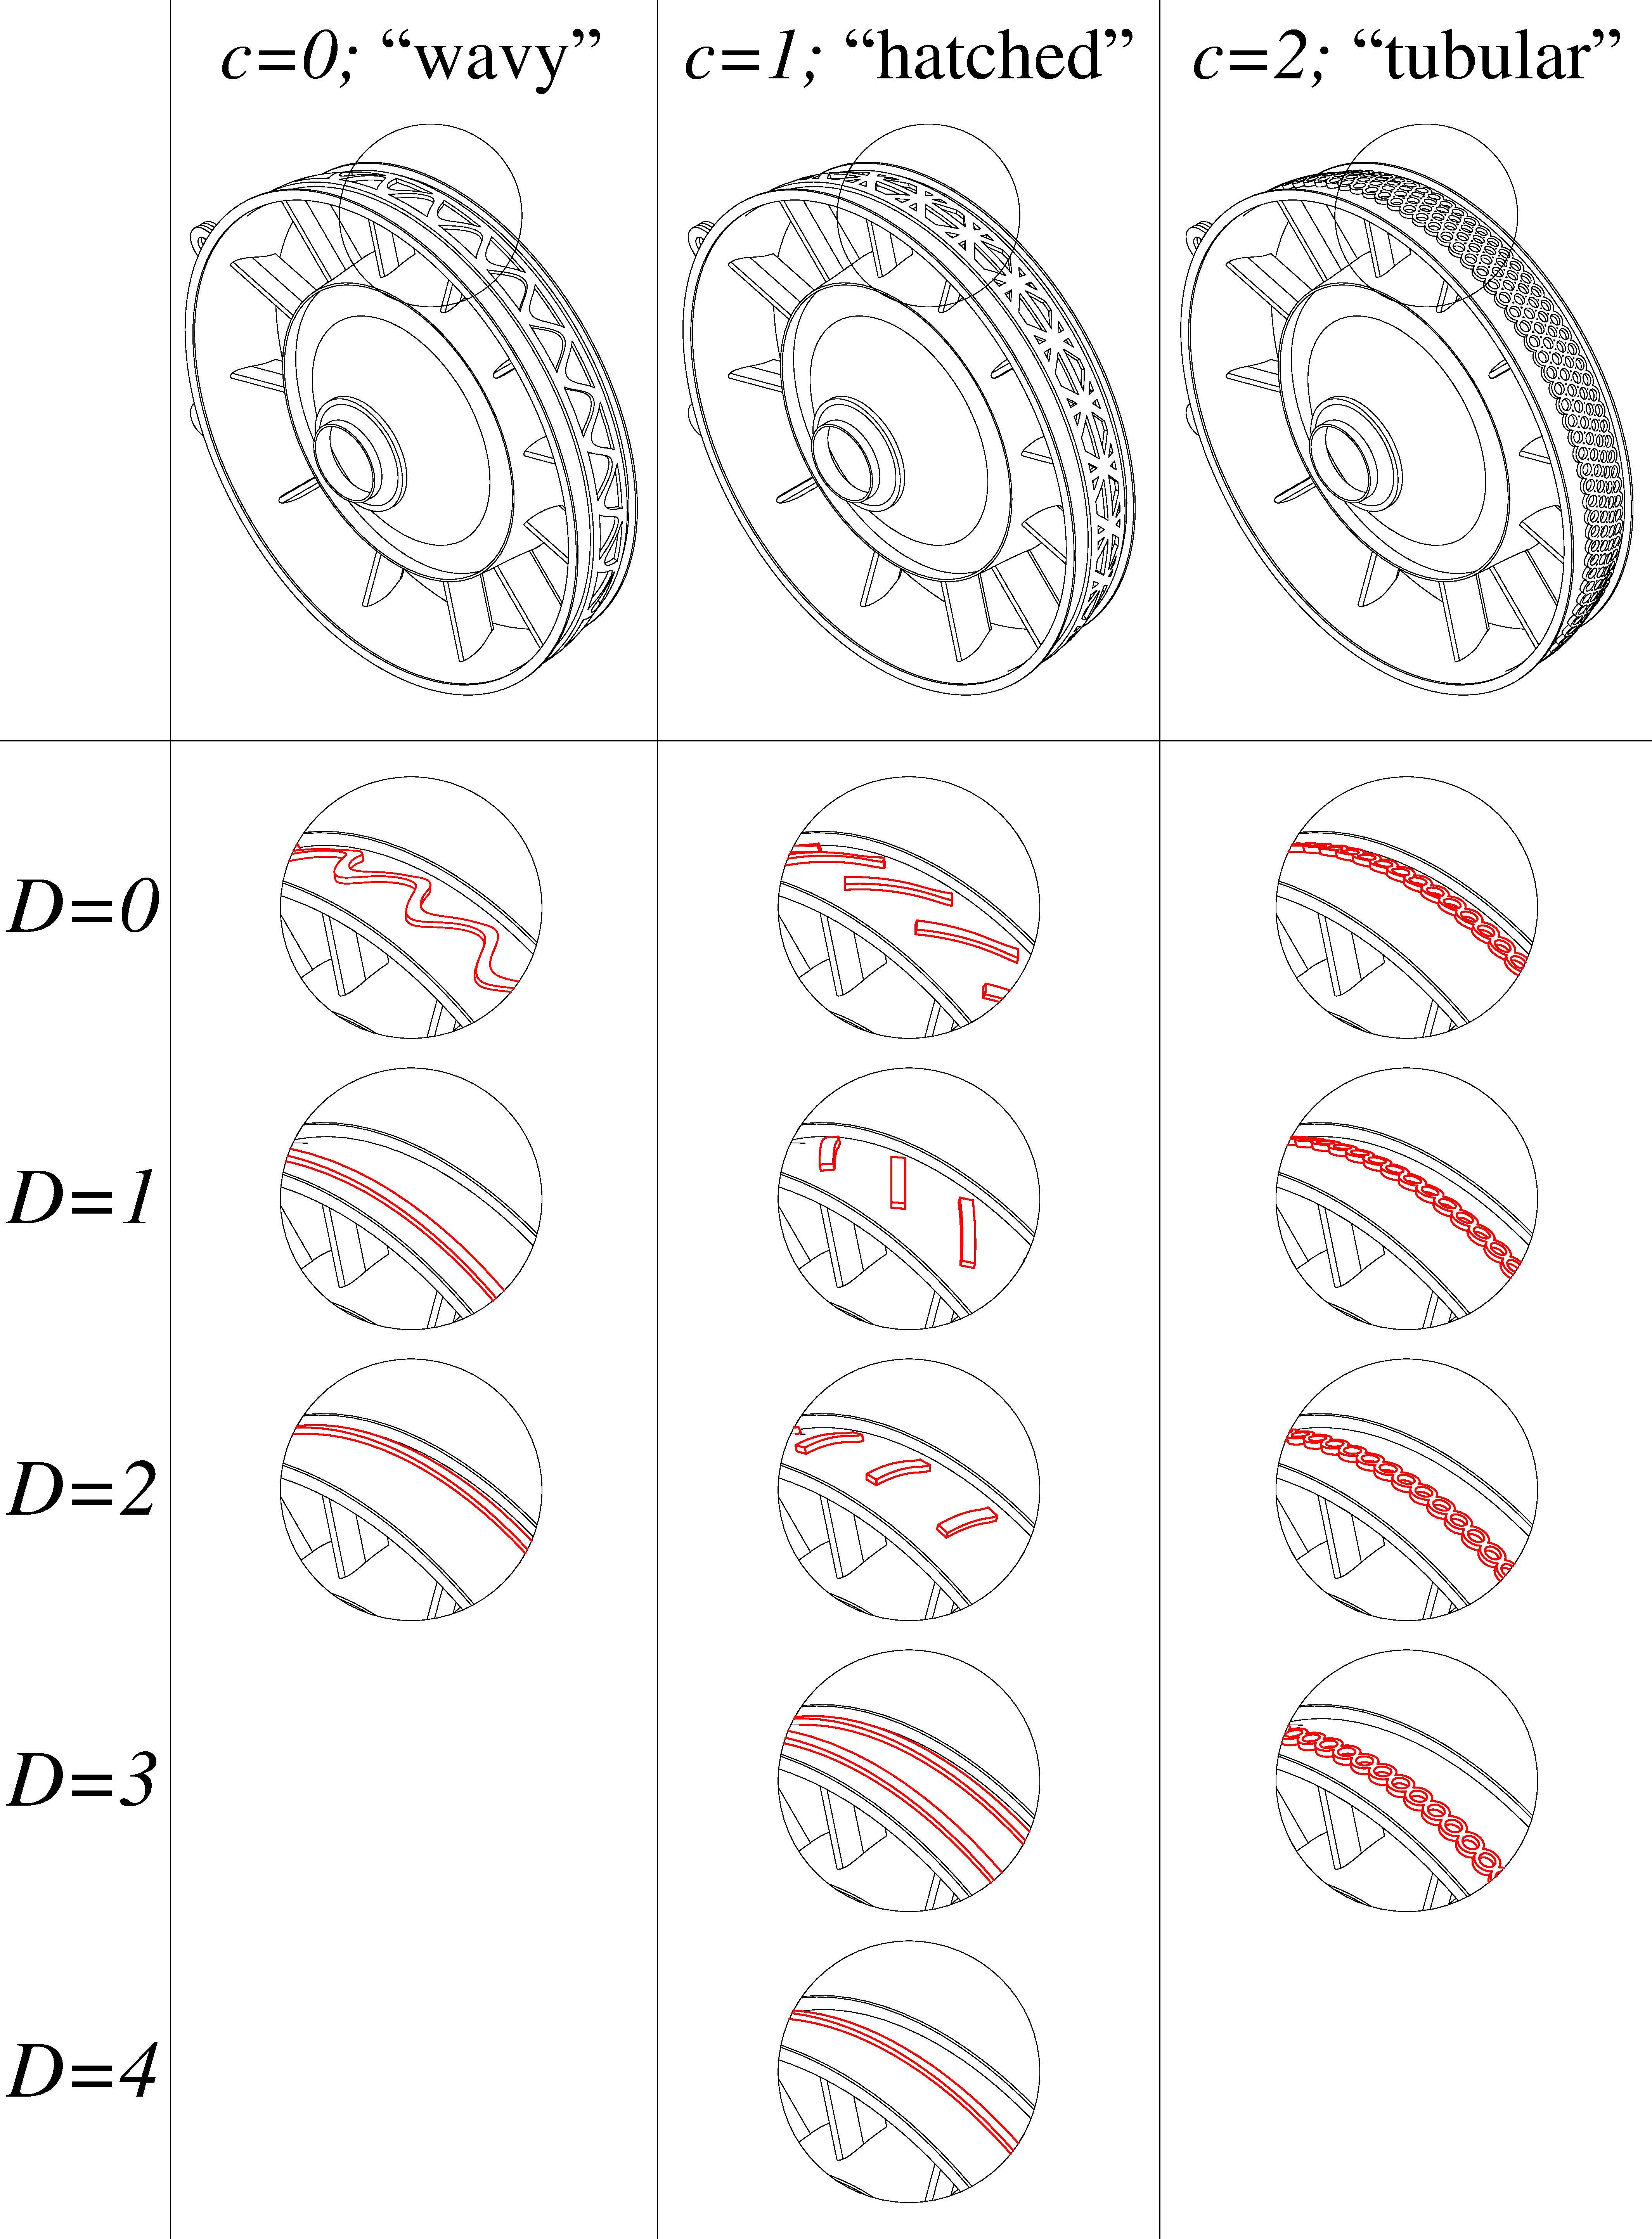
\includegraphics[width=0.6\textwidth]{6_TRS_stiffener_types.pdf}
	\caption{Illustration of possible concepts and redesign choices for \ac{TRS} stiffener}
	\label{fig:designspacestiff}
\end{figure}

We compute the cardinality of the set $\Omega_{cD}$ using Table~\ref{table:omegadcardinality} and Equation~(\ref{eq:cardinailitycdarc}) for this problem.

\begin{equation*}
	\begin{aligned}
		& \mathrm{concept~}c_0:~|\Omega_{D0}| = 15\\
		& \mathrm{concept~}c_1:~|\Omega_{D1}| = 325\\
		& \mathrm{concept~}c_2:~|\Omega_{D2}| = 64\\
		& \beta = |\Omega_{cD}| = 15 + 325 + 64 = 404.\\
	\end{aligned}
\end{equation*}

We now describe the analysis steps for obtaining the capability of a given stiffener design arc as a function of the thermal temperature loads.

%---------------------------------------------------------------------%
% Load case description
\subsection{Loadcase description} \label{subsec:loadcase}

The uncertain temperature loads in Figure~\ref{fig:thermalloads} are used to specify the vector of uncertain parameters given by $\mathbf{p} = \left[T_1 ~ T_2 ~ T_3 ~ T_4\right]^{\mathrm{T}}$ and the corresponding parameters space $\mathbf{p}\in\mathbb{R}^4$, where $n = 4$ is dimensionality of the problem. We constrain our study to a parameters space defined by the following bounds on $\mathbf{p}$.

\begin{equation*}
	\begin{aligned}
		& \mathbf{p} = \left\{\mathbf{p}: \mathbf{L} \le \mathbf{p} \le \mathbf{U}\right\},~\textrm{where}\\
		& \mathbf{L} = \left[-100 ~ -100 ~ -100 ~ -100\right]^{\mathrm{T}}~\textrm{and}\\
		& \mathbf{U} = \left[100 ~ 100 ~ 100 ~ 100\right]^{\mathrm{T}}\\
	\end{aligned}
\end{equation*}

Note that these bounds are relative to nominal temperature values of 

\begin{equation*}
	\mathbf{p}_{\textrm{nominal}} = \left[300 ~ 400 ~ 450 ~ 600\right]^{\mathrm{T}}.
\end{equation*}

A value of 

\begin{equation*}
	\begin{aligned}
		& \mathbf{p} = \left[50 ~ 25 ~ -40 ~ -20\right]^{\mathrm{T}} \equiv \\
		& \mathbf{p} + \mathbf{p}_{\textrm{nominal}} = \left[350 ~ 425 ~ 410 ~ 580\right]^{\mathrm{T}}.
	\end{aligned}
\end{equation*}

In this chapter, we assume that there is no correlation between these temperature loads. This is because environmental factors such as the atmospheric temperature are independent of the exhaust temperature. This allows us to assume that the requirement \acp{PDF} defined in Section~\ref{subsec:designmetrics} feature diagonal covariance matrices.

The feasibility of a \ac{TRS} design is governed by a single feasibility constraint $g_{f1}(\mathbf{p}) - t_1 \le 0$. For this problem, $g_{f1}(\mathbf{p}) = -n_{\textrm{safety}}(\mathbf{p})$ which is the safety factor of the design against low-cycle fatigue failure or yielding whichever comes first and is computed by a structural analysis model following the thermomechanical analysis of the stiffener deposition. $t_1 = -2.8$ is the threshold safety factor that defines feasibility. The safety factor $n_{\textrm{safety}}(\mathbf{p})$ is computed using the procedure in Section \ref{subsec:fatigueanalysis}. Note that the safety factor $n_{\textrm{safety}}(\mathbf{p})$ for a particular stiffener design arc is dependant on the applied temperature loads $(\mathbf{p})$.

For every design arc in $\Omega_{cD}$, we construct a surrogate model for computing $n_{\textrm{safety}}(\mathbf{p})$. The surrogate is constructed by training a response surface model from data obtained from the simulation model. 25 \ac{LH} samples from the parameters space are used as training data for the response surface. We use an open source surrogate model library to build and optimize the hyperparameters of an ensemble of surrogates \cite{Talgorn2018}. This results in a surrogate for the feasibility constraint $\hat{g}_{f1}(\mathbf{p}) - t_1 \le 0$. We visualize this feasibility constraint on the 4-dimensional parameters space for a few example design arcs in Section~\ref{subsec:exampleprob4D}. 

%---------------------------------------------------------------------%
% Load case requirements
\subsection{Loadcase requirements} \label{subsec:loadcasereq}

Having defined the 4-dimensional parameters space, we can now define the requirement joint \acp{PDF} that will be used and the corresponding requirement arcs that can be constructed from them. 

Two types of requirement joint \acp{PDF} will be used, the uniform distribution and the Gaussian distribution given by Equations~(\ref{eq:uniformpdf}) and (\ref{eq:gaussianpdf}), respectively. As a result, $\mathcal{T} = \left\{\mathrm{``Uniform"},\mathrm{``Gaussian"}\right\}$.

All design metrics and requirements are calculated for uncertain parameters spaces that are scaled between $0$ and $1$. This helps when making comparisons between different design arcs in terms of hypervolume of sets with $0$ being the minimum possible hypervolume and $1$ being the maximum possible hypervolume.

$e=5$ interpolation levels are used to obtain $\mathbf{M}$ and $\boldsymbol{\Sigma}$. The starting mean and interval vectors are $\boldsymbol{\mu}_1 = \left[0.15 ~ 0.80 ~ 0.80 ~ 0.85\right]^{\mathrm{T}}$ and $\boldsymbol{\sigma}_1 = \left[0.1875 ~ 0.125 ~ 0.125 ~ 0.1875\right]^{\mathrm{T}}$, respectively. The ending mean and interval vectors are $\boldsymbol{\mu}_5 = \left[0.85 ~ 0.20 ~ 0.20 ~ 0.15\right]^{\mathrm{T}}$ and $\boldsymbol{\sigma}_5 = \left[0.375 ~ 0.250 ~ 0.250 ~ 0.375\right]^{\mathrm{T}}$, respectively. As a result, the matrices of mean and interval vectors are given by

% \begin{equation*}
% 	M = \begin{Bmatrix} 
% 		[ & 0.15 & 0.80 & 0.80 & 0.85 & ],\\ 
% 		[ & 0.325 & 0.65 & 0.65 & 0.675 & ],\\
% 		[ & 0.5 & 0.5 & 0.5 & 0.5 & ],\\
% 		[ & 0.675 & 0.35 & 0.35 & 0.325 & ],\\
% 		[ & 0.85 & 0.20 & 0.20 & 0.15 & ]
% 	 \end{Bmatrix},
% \end{equation*}

% and \begin{equation*}
% 	\Sigma = \begin{Bmatrix} 
% 		[ & 0.1875 & 0.125 & 0.125 & 0.1875 & ],\\ 
% 		[ & 0.234375 & 0.15625 & 0.15625 & 0.234375 & ],\\
% 		[ & 0.28125 & 0.1875 & 0.1875 & 0.28125 & ],\\
% 		[ & 0.328125 & 0. & 0.21875 & 0.328125 & ],\\
% 		[ & 0.375 & 0.250 & 0.250 & 0.375 & ]
% 	 \end{Bmatrix}
% \end{equation*}

\begin{equation*}
	\mathbf{M} = \begin{bmatrix}
		\boldsymbol{\mu}_1 ^ {\mathrm{T}} \\ 
		\boldsymbol{\mu}_2 ^ {\mathrm{T}} \\
		\boldsymbol{\mu}_3 ^ {\mathrm{T}} \\
		\boldsymbol{\mu}_4 ^ {\mathrm{T}} \\
		\boldsymbol{\mu}_5 ^ {\mathrm{T}} 
	\end{bmatrix} = \begin{bmatrix}
		0.15 & 0.80 & 0.80 & 0.85 \\ 
		0.325 & 0.65 & 0.65 & 0.675 \\
		0.5 & 0.5 & 0.5 & 0.5 \\
		0.675 & 0.35 & 0.35 & 0.325 \\
		0.85 & 0.20 & 0.20 & 0.15 
	\end{bmatrix}
\end{equation*}

and

\begin{equation*}
	\boldsymbol{\Sigma} = \begin{bmatrix}
		\boldsymbol{\sigma}_1 ^ {\mathrm{T}} \\ 
		\boldsymbol{\sigma}_2 ^ {\mathrm{T}} \\
		\boldsymbol{\sigma}_3 ^ {\mathrm{T}} \\
		\boldsymbol{\sigma}_4 ^ {\mathrm{T}} \\
		\boldsymbol{\sigma}_5 ^ {\mathrm{T}} 
	\end{bmatrix} = \begin{bmatrix}
		0.1875 & 0.125 & 0.125 & 0.1875 \\ 
		0.234375 & 0.15625 & 0.15625 & 0.234375 \\
		0.28125 & 0.1875 & 0.1875 & 0.28125 \\
		0.328125 & 0.21875 & 0.21875 & 0.328125 \\
		0.375 & 0.250 & 0.250 & 0.375
	\end{bmatrix},
\end{equation*}

respectively.

We define a remanufacturing design problem with $m = 6$ epochs. The number of choices $v$ for $\mathcal{R} = \left\{F_{\mathbf{X}1}(\mathbf{p}),F_{\mathbf{X}2}(\mathbf{p}),\cdots,F_{\mathbf{X}v}(\mathbf{p})\right\}$ and the cardinality $s$ for $\Omega_R$ is calculated as

\begin{equation*}
	\begin{aligned}
		& v = e \times e \times |\mathcal{T}| = 5 \times 5 \times 2 = 50,~\mathrm{and}\\
		& s = |\Omega_R| = m^v = 6^{50},~\mathrm{respectively}.\\
	\end{aligned}
\end{equation*}

Only the first few elements of $\Omega_R$ will be used during the set-based design analysis and $s$ will be capped at $10^5$ samples. This is because the set-based solutions stabilize and do not change after sampling $10^3$ requirement arcs.

The reliability threshold vector for this application problem is defined as 

\begin{equation*}
    \mathbf{P}_{th} = \left[0.01 ~ 0.1 ~ 0.3 ~ 0.3 ~ 0.8 ~ 0.9\right]^{\mathrm{T}}.
\end{equation*}

The reliability threshold gradually increases as a product development cycle progresses. This is in contrast to the reliabilities encountered during a product's lifecycle where the reliability is generally high in aerospace industries. The designer can test and react to different lifecycle scenarios by adjusting the reliability threshold for the problem.

We summarize the important problem parameters and constants in Table~\ref{table:modelsummary}.

\begin{table}[h!]
	\centering
	\renewcommand{\arraystretch}{1.0}% Wider
	\footnotesize\addtolength{\tabcolsep}{-5pt}
	\caption{Relevant model parameters and constants}
	\label{table:modelsummary}
	\begin{tabular}{lcc>{\centering\arraybackslash}p{4cm}}
	\hline\hline
	\bf Parameter/constant & \bf Notation & \bf Units & \bf Nominal value \\
	\hline
	%================================================================
	Concept choices & $\mathcal{C}$ & - & $\left\{0,1,2\right\}$ \\
	Deposit choices for concept 0 & $\mathcal{D}_0$ & - & $\left\{0,1,2\right\}$ \\
	Deposit choices for concept 1 & $\mathcal{D}_1$ & - & $\left\{0,1,2,3,4\right\}$ \\
	Deposit choices for concept 2 & $\mathcal{D}_2$ & - & $\left\{0,1,2,3\right\}$ \\
	Cardinality of design arcs & $\beta$ & - & 404  \\
	Number of epochs & $m$ & - & 6 \\
	Interpolation levels & $e$ & - & 5 \\
	\ac{PDF} types & $\mathcal{T}$ & - & $\left\{\mathrm{``Uniform"},\mathrm{``Gaussian"}\right\}$ \\
	\ac{PDF} starting mean & $\boldsymbol{\mu}_1$ & - & $\left[0.15 ~ 0.80 ~ 0.80 ~ 0.85\right]^{\mathrm{T}}$ \\
	\ac{PDF} starting interval & $\boldsymbol{\sigma}_1$ & - & $\left[0.1875 ~ 0.125 ~ 0.125 ~ 0.1875\right]^{\mathrm{T}}$ \\
	\ac{PDF} ending mean & $\boldsymbol{\mu}_e$ & - & $\left[0.85 ~ 0.20 ~ 0.20 ~ 0.15\right]^{\mathrm{T}}$ \\
	\ac{PDF} ending interval & $\boldsymbol{\sigma}_e$ & - & $\left[0.375 ~ 0.250 ~ 0.250 ~ 0.375\right]^{\mathrm{T}}$ \\
	Reliability threshold & $\mathbf{P}_{th}$ & - & $\left[0.01 ~ 0.1 ~ 0.3 ~ 0.3 ~ 0.8 ~ 0.9\right]^{\mathrm{T}}$ \\
	Number of requirement \acp{PDF} & $v$ & - & 50 \\
	Number of requirement arc samples & $s$ & - & $10^5$ \\ \hline
	%================================================================
	Nacelle temperature & $T_1$ & $^{o}$C & $300 \pm 100$ \\ 
	Tailcone temperature & $T_2$ & $^{o}$C & $400 \pm 100$ \\ 
	Rotor temperature & $T_3$ & $^{o}$C & $450 \pm 100$ \\ 
	Gas surface temperature & $T_4$ & $^{o}$C & $600 \pm 100$ \\
	Parameter vector & $\mathbf{p}$ & - & $\left[T_1 ~ T_2 ~ T_3 ~ T_4\right]^{\mathrm{T}}$ \\ \hline
	%================================================================
	Laser Power & ${P_\textrm{laser}}$ & W &  3806 \\ 
	Laser beam radius & ${r_l}$ & mm & 14.2 \\ 
	Scanning speed& ${V}$ & mm/s & 5.0 \\ 
	Stiffener height & $S_\textrm{height}$ & mm & 10.0 \\
	Laser penetration depth & $D_p$ & mm & 5.0 \\
	Number of deposition layers & $n_d$ & - & 2 \\
	Threshold low-cycle fatigue safety factor & $t_1$ & - & -2.8 \\
	%================================================================
	\hline\hline
	\end{tabular}
\end{table}

%============================ RESULTS ============================%
\section{Results and discussion} \label{sec:TSEresults}

% {\color{red} Here we describe the obtained results in the context of a tradespace and comment on the most frequent deposit type encountered during the first stage. This helps designers choose a good starting point that will allow room to evolve to meet the largest number of possible requirement profiles likely to be encountered in the future}

We investigate the remanufacturing design problem of a \ac{TRS} by using the surrogate thermomechanical/structural analysis to obtain the capability set for every design arc in the set $\Omega_{cD}$. We begin by investigating a few select design arcs from $\Omega_{cD}$. We then solve a single combinatorial optimization problem to minimize excess for a given requirement arc from the set $\Omega_R$. We then present the set-based results for the problem using a tradespace.

%---------------------------------------------------------------------%
% Example calculation
\subsection{Example for calculating the design properties of a given design arc} \label{subsec:exampleprob4D}

The requirements are defined in the parameters space by either a uniform or Gaussian \ac{PDF} given by Equations~(\ref{eq:uniformpdf}) and (\ref{eq:gaussianpdf}), respectively. We choose two design arcs from the set $\Omega_{cD}$ to visualize their feasibility constraints, capabilities, and reliabilities in the 4-dimensional parameters space in Figure~\ref{fig:4Dexamplepspace}. The design arcs and their filtered outdegree, weight, and hypervolume of capability are reported in Table~\ref{table:pdf4Dexample}. Additionally, two different requirement joint \acp{PDF} are specified and the corresponding reliability, hypervolume of requirement and hypervolume of excess are reported in Table~\ref{table:pdf4Dexample}.

\newcommand{\cwaa}{0.75cm} % index column width
\newcommand{\cwa}{1.5cm} % design arc column width
\newcommand{\cwc}{1.5cm} % FO column width
\newcommand{\cwd}{1cm} % FO column width
\newcommand{\cwe}{1.5cm} % mean column width
\newcommand{\cwf}{1.5cm} % interval column width
%
%
\newcommand{\cwb}{1.1cm} % Capability column width
\newcommand{\cwi}{1.1cm} % R volume column width
\newcommand{\cwj}{1.1cm} % E volume column width

\begin{table}[h!]
	\centering
	% \renewcommand{\arraystretch}{1.0}% Wider
	\footnotesize\addtolength{\tabcolsep}{-5pt}
	\caption{Results obtained for example design arcs and requirement joint \acp{PDF}}
	\label{table:pdf4Dexample}
	\begin{tabular}{>{\centering\arraybackslash}p{\cwaa}>{\centering\arraybackslash}p{\cwa}|>{\centering\arraybackslash}p{\cwc}c>{\centering\arraybackslash}p{\cwe}>{\centering\arraybackslash}p{\cwf}cc>{\centering\arraybackslash}p{\cwi}>{\centering\arraybackslash}p{\cwj}>{\centering\arraybackslash}p{\cwb}}
	\hline\hline
	\bf Index & \bf Design arc & \bf Filtered outdegree & \bf Weight &\bf \ac{PDF} mean vector & \bf \ac{PDF} interval vector & \bf \ac{PDF} type & \bf Reliability & \multicolumn{3}{c}{\bf Set volume} \\
	$\lambda$ & $\left\{c,\mathbf{D}\right\}$ & $FO$ & $W$ &$\boldsymbol{\mu}$ & $\boldsymbol{\sigma}$ & $t$ & $\mathbb{P}\left(\mathbf{p}\in C\right)$ & $V_R$ & $V_E$ & $V_C$ \\ \hline
	%================================================================
	\multirow{5}{\cwaa}{\centering 109} & & \multirow{5}{\cwc}{\centering 2} & \multirow{5}{\cwd}{\centering 13.9 kg} & \multirow{5}{\cwe}{\centering $\begin{bmatrix} 0.375 \\ 0.5 \\ 0.5 \\0.625 \end{bmatrix}$} & \multirow{5}{\cwf}{\centering $\begin{bmatrix} 0.375 \\ 0.125 \\ 0.125 \\0.375 \end{bmatrix}$} & & & & & \multirow{5}{\cwb}{\centering 0.540} \\
	 & $\{c = 1,$ & & & & & ``Uniform" & 0.3089 & 0.0352 & 0.529 \\
	 & $\mathbf{D} = \left[1,2,4\right]\}$ & & & & & & & & & \\
	 & & & & & & ``Gaussian" & 0.165 & 0.0108 & 0.540\\
	 & & & & & & & & & & \\ \hline
	%================================================================
	\multirow{5}{\cwaa}{\centering 110} & & \multirow{5}{\cwc}{\centering 1} & \multirow{5}{\cwd}{\centering 18.5 kg} & \multirow{5}{\cwe}{\centering $\begin{bmatrix} 0.375 \\ 0.5 \\ 0.5 \\0.625 \end{bmatrix}$} & \multirow{5}{\cwf}{\centering $\begin{bmatrix} 0.375 \\ 0.125 \\ 0.125 \\0.375 \end{bmatrix}$} & & & & & \multirow{5}{\cwb}{\centering 0.883} \\
	 & $\{c = 1,$ & & & & & ``Uniform" & 0.759 & 0.0352 & 0.856 \\
	 & $\mathbf{D} = \left[1,2,4,0\right]\}$ & & & & & & & & & \\
	 & & & & & & ``Gaussian" & 0.908 & 0.0108 & 0.875 \\
	 & & & & & & & & & & \\
	%================================================================
	\hline\hline
	\end{tabular}
\end{table}

We can see from the results in Table~\ref{table:pdf4Dexample} that the addition of one more deposit to the design arc $\left\{c = 1, \mathbf{D} = \left[1,2,4\right]\right\}$ increases its performance in terms of capability and reliability. However, this comes at the increased cost of an additional 4.6 kg of weight, reduced filtered outdegree, and an additional excess of 0.327 and 0.335 for uniform and Gaussian \acp{PDF}, respectively. The choice of design arc for a given requirement arc is driven by the need to maintain a minimum reliability while minimizing excess. We will look at such a problem using epoch-era analysis and combinatorial optimization for decision making.

\begin{figure}[h!]
	\centering
	\subfloat[{$\left\{c = 1,\mathbf{D} = \left[1,2,4\right]\right\}$}\label{fig:darc1R1}]{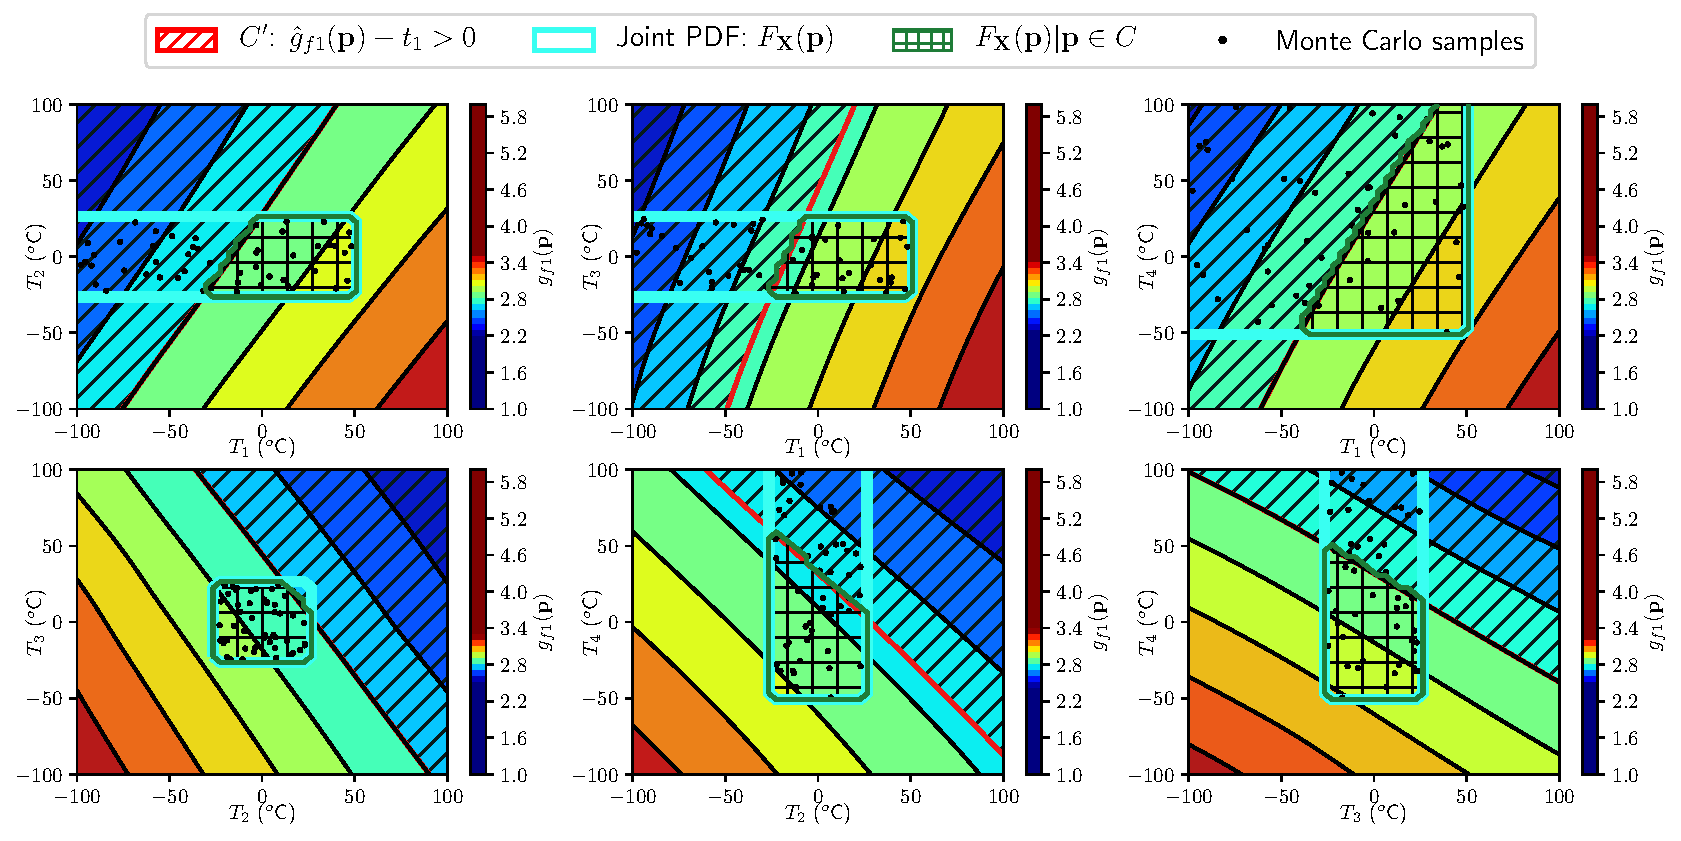
\includegraphics[width=0.9\textwidth]{8a_thermal_out_nominal_RS}}
	
	\subfloat[{$\left\{c = 1,\mathbf{D} = \left[1,2,4,0\right]\right\}$} \label{fig:darc2R1}]{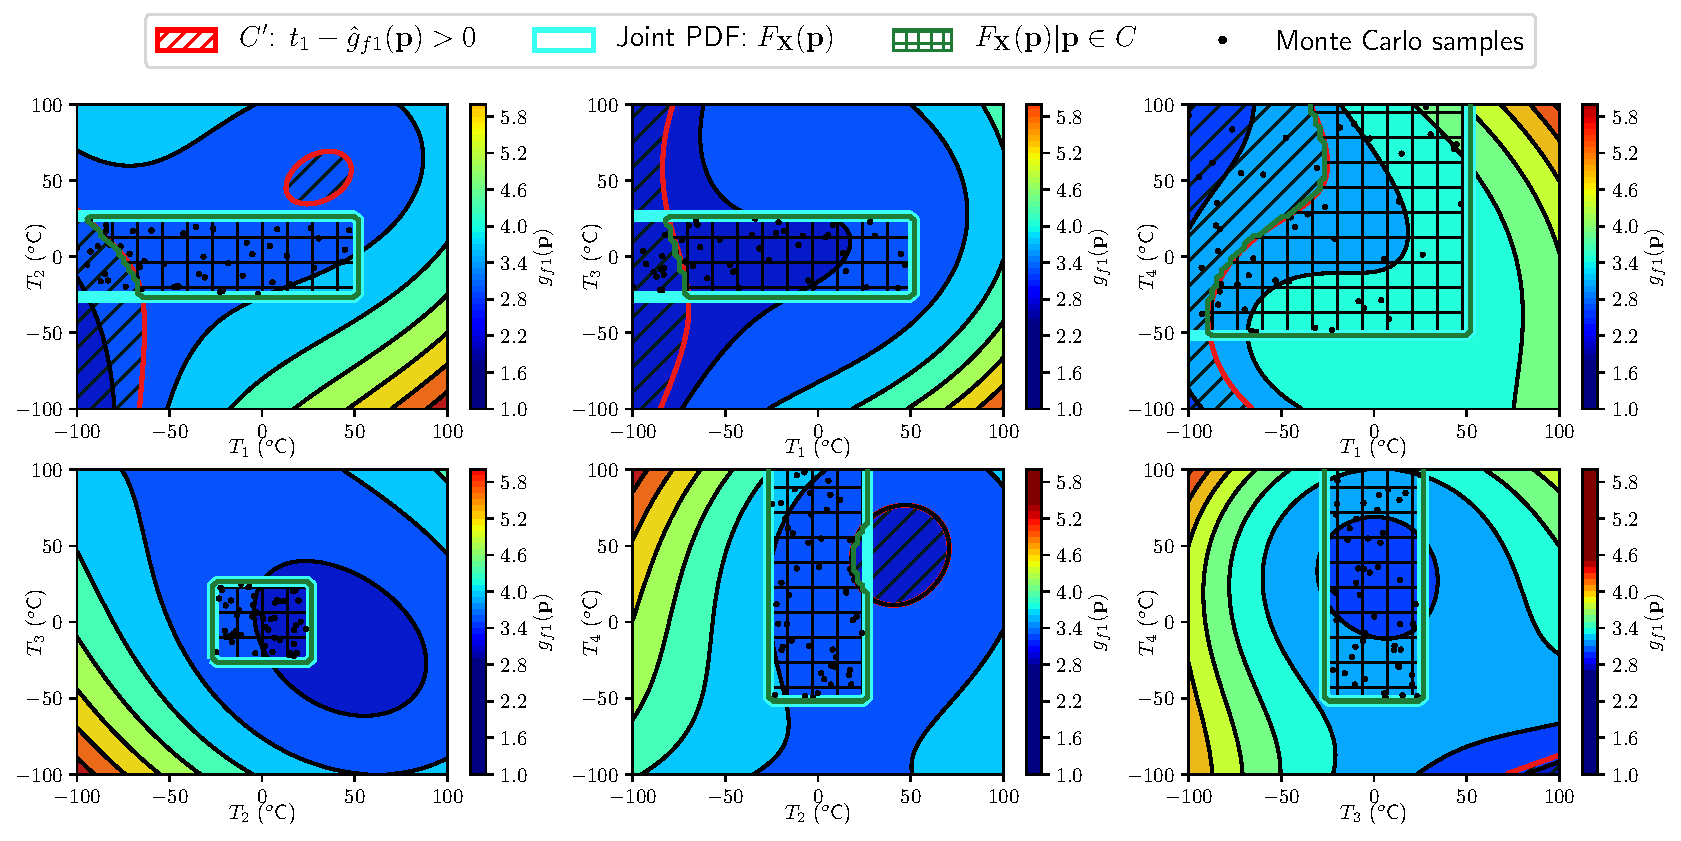
\includegraphics[width=0.9\textwidth]{8b_thermal_out_nominal_RS}}
	\caption{2D projections of the parameters space $\mathbf{p} \in \mathbb{R}^4$}
	\label{fig:4Dexamplepspace}
\end{figure}

%---------------------------------------------------------------------%
% Example calculation
\subsection{Combinatorial optimization with respect to a requirement arc} \label{subsec:exampleoptprob}

We solve the problem given by Equation~(\ref{eq:TSEoptproblem}) using \ac{MADS} for mixed variable problems \cite{Abramson2009}. The requirement arc $\mathbf{R}_w$ used for this problem is given in Table~\ref{table:requirementarcex}. The probability threshold used to define the reliability constraints is given as

\begin{equation*}
    \mathbf{P}_{th} = \left[0.01~0.1~0.3~0.3~0.8~0.9\right]^{\mathrm{T}}.
\end{equation*}

\begin{table}[h!]
	\centering
	\renewcommand{\arraystretch}{1.0}% Wider
	\footnotesize\addtolength{\tabcolsep}{-5pt}
	\caption{Requirement arc $\mathbf{R}_w$ details$^*$}
	\label{table:requirementarcex}
	\begin{tabular}{l>{\centering\arraybackslash}p{4.2cm}>{\centering\arraybackslash}p{6cm}c}
	\hline\hline

	\bf \ac{PDF} Index & \bf \ac{PDF} mean vector & \bf \ac{PDF} interval vector & \bf \ac{PDF} type \\
	$F_\mathbf{X} \in \mathcal{R}$ &$\boldsymbol{\mu}$ & $\boldsymbol{\sigma}$ & $t$ \\ \hline

	\hline
	%================================================================
	$F_{\mathbf{X36}}$ & $\begin{bmatrix} 0.5 & 0.5 & 0.5 & 0.5 \end{bmatrix}$ & $\begin{bmatrix} 0.1875 & 0.125 & 0.125 & 0.1875 \end{bmatrix}$ & "Gaussian" \\
	$F_{\mathbf{X50}}$ & $\begin{bmatrix} 0.85 & 0.2 & 0.2 & 0.15 \end{bmatrix}$ & $\begin{bmatrix} 0.375 & 0.25 & 0.25 & 0.375 \end{bmatrix}$ & "Gaussian" \\
	$F_{\mathbf{X1}}$ & $\begin{bmatrix} 0.15 & 0.8 & 0.8 & 0.85 \end{bmatrix}$ & $\begin{bmatrix} 0.1875 & 0.125 & 0.125 & 0.375 \end{bmatrix}$ & "uniform" \\
	$F_{\mathbf{X46}}$ & $\begin{bmatrix} 0.85 & 0.2 & 0.2 & 0.15 \end{bmatrix}$ & $\begin{bmatrix} 0.1875 & 0.125 & 0.125 & 0.1875 \end{bmatrix}$ & "Gaussian" \\
	$F_{\mathbf{X13}}$ & $\begin{bmatrix} 0.5 & 0.5 & 0.5 & 0.5 \end{bmatrix}$ & $\begin{bmatrix} 0.28125 & 0.1875 & 0.1875 & 0.28125 \end{bmatrix}$ & "uniform" \\
	$F_{\mathbf{X31}}$ & $\begin{bmatrix} 0.325 & 0.65 & 0.65 & 0.675 \end{bmatrix}$ & $\begin{bmatrix} 0.1875 & 0.125 & 0.125 & 0.1875 \end{bmatrix}$ & "Gaussian" \\
	%================================================================
	\hline\hline
	\end{tabular}\\
	\footnote[1]{}The transpose operator $^{\mathrm{T}}$ is dropped to avoid repetition
\end{table}

We plot the results from various decision arcs across epochs in Figure~\ref{fig:epocheraexample}. The first decision arc, $\left\{c=1,\mathbf{S}=\left[2,1,-1,-1,0,-1\right]\right\}$ (shown in red) does not satisfy the reliability constraints for the problem as shown in Figure~\ref{fig:Decisionarcreliability}. This is because for epoch $k=3$, the reliability of the corresponding design arc $\left\{c=1,\mathbf{D}=\left[2,1\right]\right\}$ is almost 0. No redesign occurred for epoch $k=3$ when it was needed to increase the reliability of the design arc above the threshold.

We investigate another decision arc $\left\{c=1,\mathbf{S}=\left[4,1,0,2,-1,3\right]\right\}$ (shown in green) that achieves very high reliability throughout all epochs. However, this comes at the cost of increased cumulative excess (green shaded area under excess/epoch graph) relative to that of the first decision arc (shown as the red shaded area) in Figure~\ref{fig:Decisionarcexcess}.

we solve the combinatorial problem given by Equation~(\ref{eq:TSEoptproblem}) to get the third decision arc $\left\{c=1,\mathbf{S}=\left[4,1,0,2,-1,3\right]\right\}$ (shown in blue) which is optimal in terms of minimizing excess. This decision arc has lower reliability relative to the second decision arc (shown in green) but lower cumulative excess and therefore less overdesign. We provide the values of the objective function and reliability constraints for all three decision arcs in Table~\ref{table:optresultsEA}.

\begin{figure}[h!]
	\centering
	\subfloat[Reliability over multiple epochs \label{fig:Decisionarcreliability}]{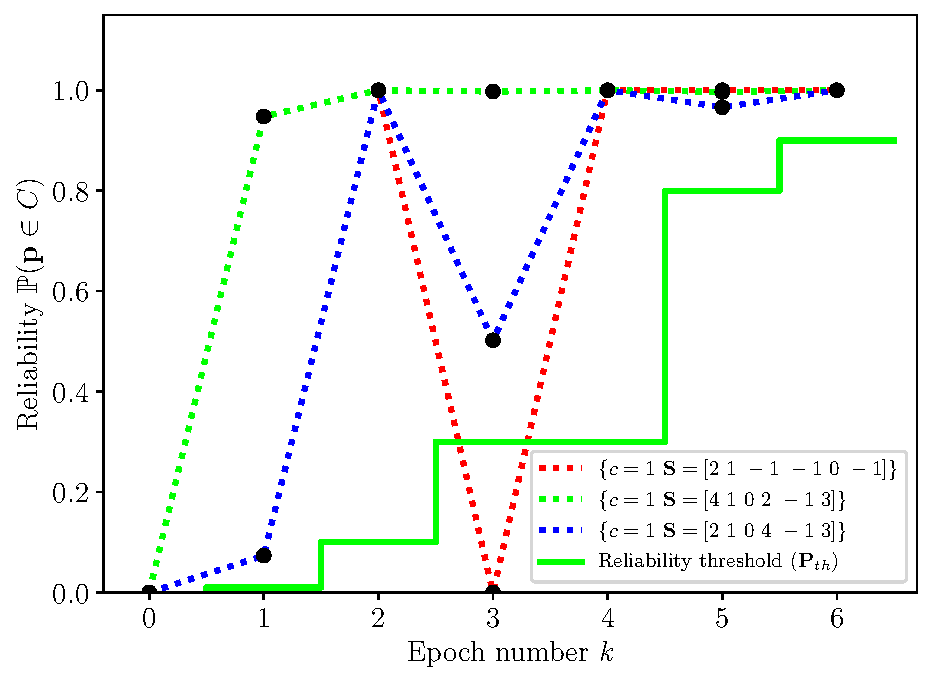
\includegraphics[width=0.45\textwidth]{10a_stagespace_res}} \hspace{0.1\textwidth}%
	\subfloat[Volume of excess set over multiple epochs \label{fig:Decisionarcexcess}]{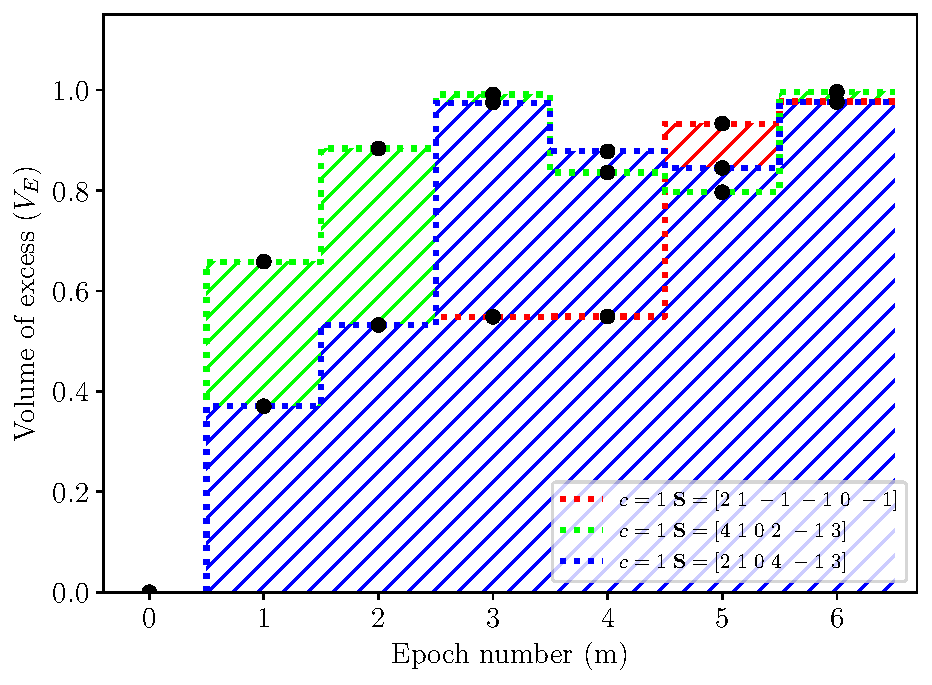
\includegraphics[width=0.45\textwidth]{10b_stagespace_obj}} \hspace{0.1\textwidth}%	
	\caption{Visualization of several decision arcs}
	\label{fig:epocheraexample}
\end{figure}

\newcommand{\ocwa}{0.75cm} % index column width
\newcommand{\ocwb}{4cm} % decision arc column width
\newcommand{\ocwc}{1.5cm} % objective column width
\newcommand{\ocwd}{2cm} % constraints column width
\newcommand{\ocwe}{3cm} % design arc column width

\begin{table}[h!]
	\centering
	% \renewcommand{\arraystretch}{1.0}% Wider
	\footnotesize\addtolength{\tabcolsep}{-5pt}
	\caption{Results obtained for example decision arcs given a requirement arc $\mathbf{R}_w$}
	\label{table:optresultsEA}
	\begin{tabular}{>{\centering\arraybackslash}p{\ocwa}>{\centering\arraybackslash}p{\ocwb}|>{\centering\arraybackslash}p{\ocwc}>{\centering\arraybackslash}p{\ocwd}>{\centering\arraybackslash}p{\ocwe}}
	\hline\hline
	\bf Index & \bf Decision arc & \bf Objective value & \bf Reliability constraints & \bf Design arc \\ & $\left\{c,\mathbf{S}\right\}$ & $f(c,\mathbf{S};\mathbf{R})$ & $\mathbf{g}(c,\mathbf{S};\mathbf{R})$ & $\left\{c,\mathbf{D}\right\}$ \\ \hline
	%================================================================
	\multirow{6}{\ocwa}{\centering 1} & & \multirow{6}{\ocwc}{\centering 3.91} & \multirow{6}{\ocwd}{\centering $\begin{bmatrix} -0.063 \\ -0.9 \\ 0.3 \\ -0.7 \\ -0.2 \\ -0.1 \end{bmatrix}$} & \\
	 & & & & \\
	 & $\{c=1,$ & & & $\{c=1,$ \\
	 & $\mathbf{S}=\left[2,1,-1,-1,0,-1\right]\}$ & & & $\mathbf{D}=\left[2,1,0\right]\}$ \\
	 & & & & \\
	 & & & & \\ \hline
	%================================================================
	\multirow{6}{\ocwa}{\centering 2} & & \multirow{6}{\ocwc}{\centering 5.16} & \multirow{6}{\ocwd}{\centering $\begin{bmatrix} -0.94 \\ -0.9 \\ -0.70 \\ -0.7 \\ -0.20 \\ -0.1 \end{bmatrix}$} & \\
	& & & & \\
	& $\{c=1,$ & & & $\{c=1,$ \\
	& $\mathbf{S}=\left[4,1,0,2,-1,3\right]\}$ & & & $\mathbf{D}=\left[4,1,0,2,3\right]\}$ \\
	& & & & \\
	& & & & \\ \hline
	%================================================================
	\multirow{6}{\ocwa}{\centering 3} & & \multirow{6}{\ocwc}{\centering 4.58} & \multirow{6}{\ocwd}{\centering $\begin{bmatrix} -0.063 \\ -0.9 \\ -0.20 \\ -0.7 \\ -0.17 \\ -0.1 \end{bmatrix}$} & \\
	& & & & \\
	& $\{c=1,$ & & & $\{c=1,$ \\
	& $\mathbf{S}=\left[2,1,0,4,-1,3\right]\}$ & & & $\mathbf{D}=\left[2,1,0,4,3\right]\}$ \\
	& & & & \\
	& & & & \\
	%================================================================
	\hline\hline
	\end{tabular}
\end{table}

Finally, the example in this section shows that the order of redesign steps can have a significant impact on the reliability and level of overdesign throughout epochs. The second and third decision arcs contain the same redesign choices but in different order. The differences between them in terms of reliability and cumulative excess reflect the importance of choosing the right order of redesign operations when considering multiple epochs.

We will now solve similar combinatorial optimization problems for every requirement arc in the set $\Omega_R$ to obtain a set-based solution.

%---------------------------------------------------------------------%
% Example calculation
\subsection{Set-based design and tradespace exploration} \label{subsec:SBDTSE}

We solve an optimization problem similar to the one in Section~\ref{subsec:exampleoptprob} for every requirement arc in $\Omega_R$ to obtain the set of parametric optimal design arcs when optimizing for cumulative excess ($S_E^*$) and cumulative weight ($S_W^*$). We plot the frequency of each design arc in $S_E^*$ and $S_W^*$ and normalize it by the cardinality $s$ of set $\Omega_R$ to obtain the histograms shown in Figure~\ref{fig:histogramplotsSBD}. 

We also evaluated the flexibility and robustness of each design arc in $\Omega_{cD}$ using the methodology in Figure~\ref{fig:methodology} and Algorithm~\ref{algo:SBDRobustalgo}. We present the set of design arcs ordered with respect to robustness and flexibility in Figures~\ref{fig:histogramR} and \ref{fig:histogramF}, respectively.

\begin{figure}[h!]
	\centering
	\subfloat[Objective: minimize cumulative excess\label{fig:histogramSBDE}]{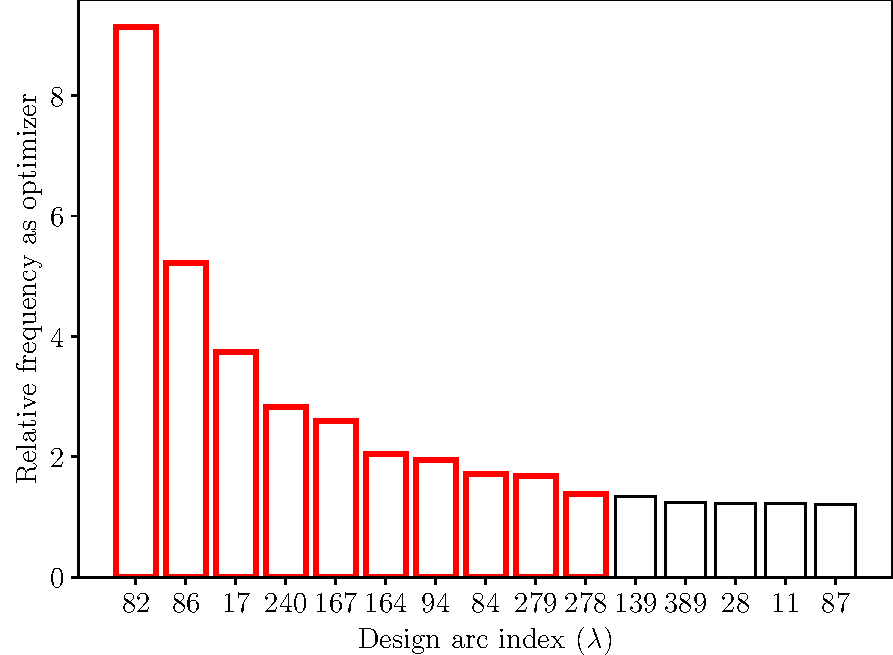
\includegraphics[width=0.45\textwidth]{11a_histogram_DOE_E}} \hspace{0.1\textwidth}%
	\subfloat[Objective: minimize cumulative weight\label{fig:histogramSBDW}]{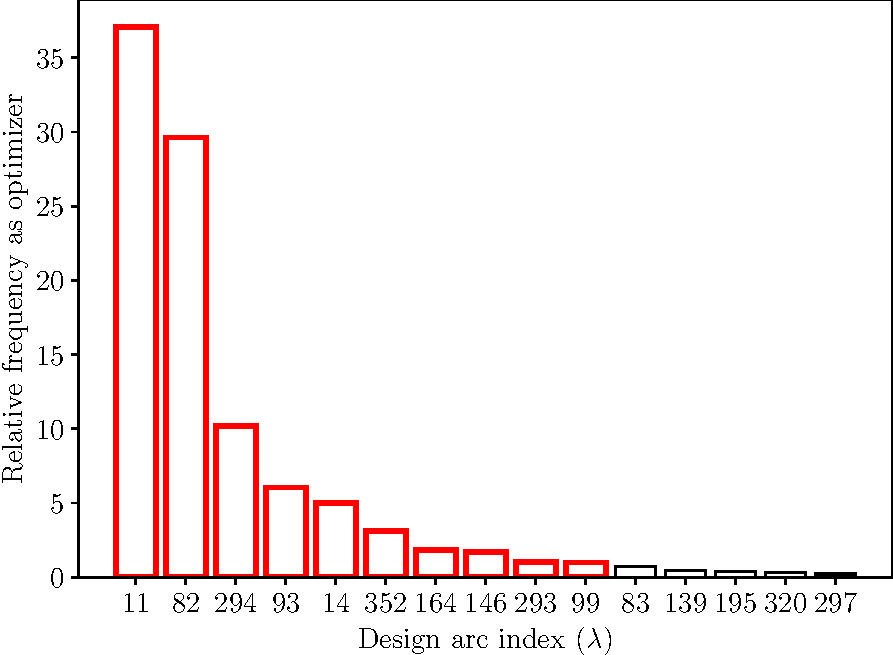
\includegraphics[width=0.45\textwidth]{11b_histogram_DOE_W}} \hspace{0.1\textwidth}%	
	\caption{Distribution of design arcs in optimization driven set-based solutions}
	\label{fig:histogramplotsSBD}
\end{figure}

\begin{figure}[h!]
	\centering
	\subfloat[Set of robust design arcs \label{fig:histogramR}]{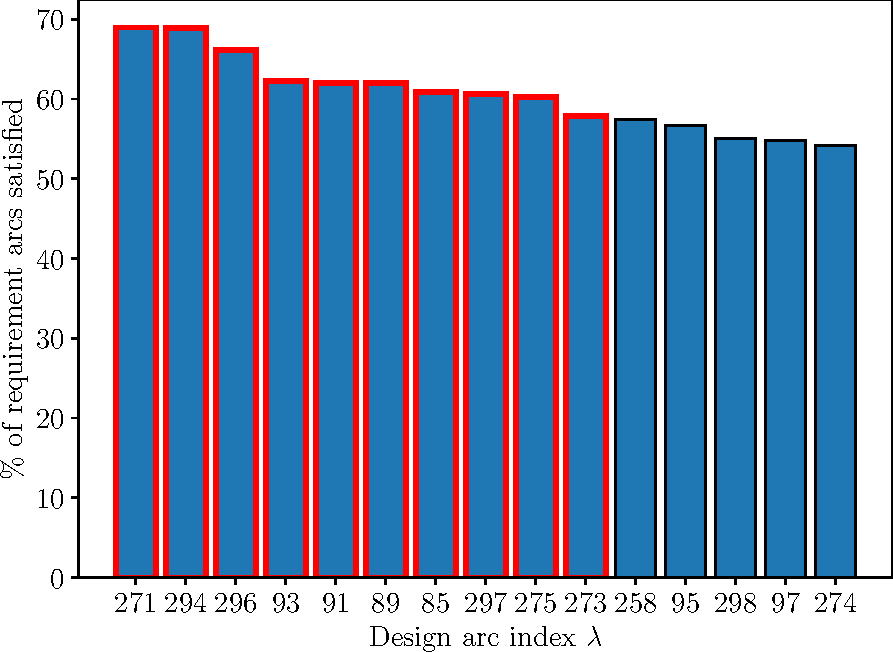
\includegraphics[width=0.45\textwidth]{12a_histogram_DOE_R}} \hspace{0.1\textwidth}%	
	\subfloat[Set of flexible design arcs \label{fig:histogramF}]{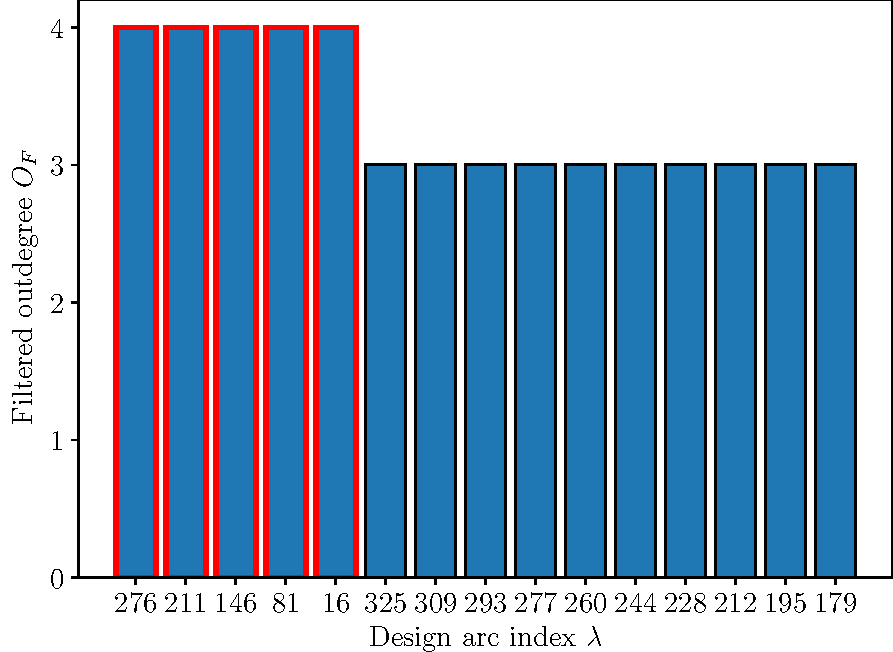
\includegraphics[width=0.45\textwidth]{12b_histogram_DOE_F}} \hspace{0.1\textwidth}%	
	\caption{Distribution of design arcs in robust and flexible set-based solutions}
	\label{fig:histogramplots}
\end{figure}

We highlight the top $\alpha = 10$ design arcs in Figures~\ref{fig:histogramplotsSBD} and \ref{fig:histogramplots} for visualization on a tradespace. A tradespace with the utility given by the volume of the capability set $V_c$ and weight $W$ is shown in Figure~\ref{fig:tradespaceSBD}. The Pareto front for the tradespace is obtained by solving the problem in Equation~(\ref{eq:optproblembiobj}).

\begin{figure}[h!]
	\centering
	\subfloat[Set-based design arcs objective: minimize cumulative excess\label{fig:tradespaceSBDE}]{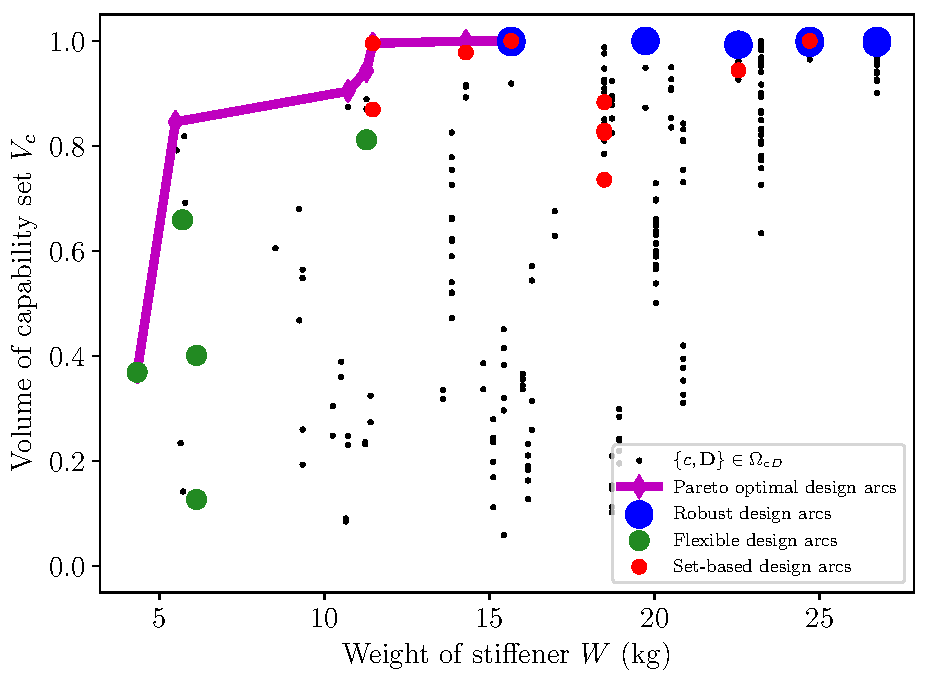
\includegraphics[width=0.45\textwidth]{13a_tradespace_pareto_E}} \hspace{0.1\textwidth}%
	\subfloat[Set-based design arcs: minimize cumulative weight\label{fig:tradespaceSBDW}]{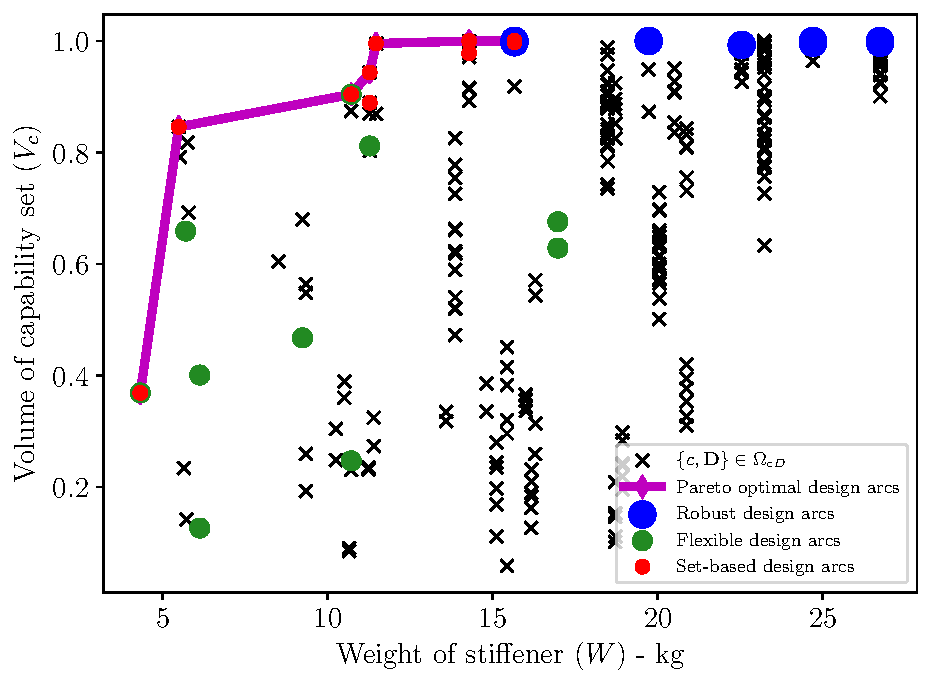
\includegraphics[width=0.45\textwidth]{13b_tradespace_pareto_W}} \hspace{0.1\textwidth}%	
	\caption{Tradespace with design arcs projected}
	\label{fig:tradespaceSBD}
\end{figure}

From the tradespace, we can draw several insights. The flexible set-based solution minimizes cost but also minimizes utility. In contrast, the robust design set maximizes utility but also maximizes the cost. The set-based solution obtained by optimization with respect to excess or weight balances utility with cost. The weight optimized set-based solution has a larger spread than the excess optimized solution. We quantify the size of the set-based solutions by their convex hulls. We use the convex hull to calculate three metrics: the area spanned by the set, location of the set given by its centroid and proximity to the Pareto front given by the distance from the centroid to the nearest Pareto point \cite{Brown2019}.

We report the convex hull metrics in Table~\ref{table:convexhullresults}.

\begin{table*}[h!]
	\centering
	\footnotesize\addtolength{\tabcolsep}{-2pt}
	\caption{Set-based solution comparison}
	\label{table:convexhullresults}
	\begin{tabular}{>{\arraybackslash}p{1.8cm}|C{1cm}C{1cm}|C{1cm}C{1cm}|C{1cm}C{1cm}|C{1cm}C{1cm}|C{1cm}C{1cm}}
		\toprule\toprule
		\multirow{2}{2cm}{\textbf{Quantity}} & \multicolumn{2}{c|}{Set of feasible} & \multicolumn{2}{c|}{Set of robust} & \multicolumn{2}{c|}{Set of flexible} & \multicolumn{2}{c|}{Set of optimal} & \multicolumn{2}{c}{Set of optimal}\\ 
		 & \multicolumn{2}{c|}{design arcs $\Omega_{cD}$} & \multicolumn{2}{c|}{design arcs $S_R$} & \multicolumn{2}{c|}{design arcs $S_F$} & \multicolumn{2}{c|}{design arcs $S_E$} & \multicolumn{2}{c}{design arcs $S_W$}\\ \hline
		%================================================================
		Coordinates & $W$ & $V_c$ & $W$ & $V_c$ & $W$ & $V_c$ & $W$ & $V_c$ & $W$ & $V_c$\\
		\hline
		Lower & 4.32 & 0.059 & 15.66 & 0.992 & 4.32 & 0.127 & 11.47 & 0.736 & 4.32 & 0.369\\
		Upper & 26.74 & 1.00 &  26.74 & 1.00 & 16.97 & 0.904 & 24.70 & 1.00 & 15.66 & 1.00\\
		Set centroid & 14.02 & 0.533 & 22.34 & 0.998 & 10.22 & 0.516 & 16.35 & 0.920 & 11.15 & 0.868 \\ \hline
		%================================================================
		$V_{\textrm{hyper-rectangle}}$ & \multicolumn{2}{c}{1} & \multicolumn{2}{c}{0.0038} & \multicolumn{2}{c}{0.466} & \multicolumn{2}{c}{0.166} & \multicolumn{2}{c}{0.339}\\
		$V_{\textrm{convhull}}$ & \multicolumn{2}{c}{0.758} & \multicolumn{2}{c}{0.0026} & \multicolumn{2}{c}{0.245} & \multicolumn{2}{c}{0.104} & \multicolumn{2}{c}{0.126}\\
		$\%V_{\textrm{feasible}}$ & \multicolumn{2}{c}{75.8\%} & \multicolumn{2}{c}{0.26\%} & \multicolumn{2}{c}{24.5\%} & \multicolumn{2}{c}{10.4\%} & \multicolumn{2}{c}{12.6\%}\\ \hline
		%================================================================
		$D_{\textrm{Pareto}}$ & \multicolumn{2}{c}{0.421} & \multicolumn{2}{c}{0.298} & \multicolumn{2}{c}{0.306} & \multicolumn{2}{c}{0.0904} & \multicolumn{2}{c}{0.0432}\\ 
		%================================================================
		\toprule\toprule
	\end{tabular}
\end{table*}

From Table~\ref{table:convexhullresults} we can see that the set of optimal design arcs with respect to cumulative excess $S_E$ occupies $10.4\%$ of the objective space which is less than that occupied by the set of flexible design arcs $S_F$ and greater than that occupied by the set of robust design arcs $S_R$. The set of optimal design arcs with respect to cumulative weight $S_W$ occupies $12.6\%$ which is comparable to the volume of $S_E$.

Furthermore, we can see that the sets of optimal design arcs $S_E$ and $S_W$ are close to the Pareto front which is expected since these sets aim to balance robustness with flexibility which are indirectly related to capability and weight.

Although there are a lot of commonalities between sets $S_E$ and $S_W$, there are some notable differences. Set $S_E$ favors designs that have higher capability when compared to $S_W$ as given by the $V_c$ coordinate of their centroids of 0.920 and 0.868, respectively. The discrepancy between the two sets is due to the fact that weight, or in more general cases, cost does not necessarily translate to excess. For example two designs of identical weight may have different excesses due to differences in the placement of the stiffener. It is therefore important that the designers carefully select their desired metric for optimization in the problem given by Equation~(\ref{eq:TSEoptproblem}).

We aim to analyze the top 6 designs in sets $S_E$ and $S_W$ in Figure~\ref{fig:histogramplotsSBD} by using the reduced tradespace shown in Figure~\ref{fig:reducedTSE}. We also display the geometry of the deposits that belong to these designs in Tables~\ref{table:depositionsequence_SE} and \ref{table:depositionsequence_SW}.

\begin{figure}[h!]
	\centering
	\subfloat[$S_E$\label{fig:reducedTSE_SE}]{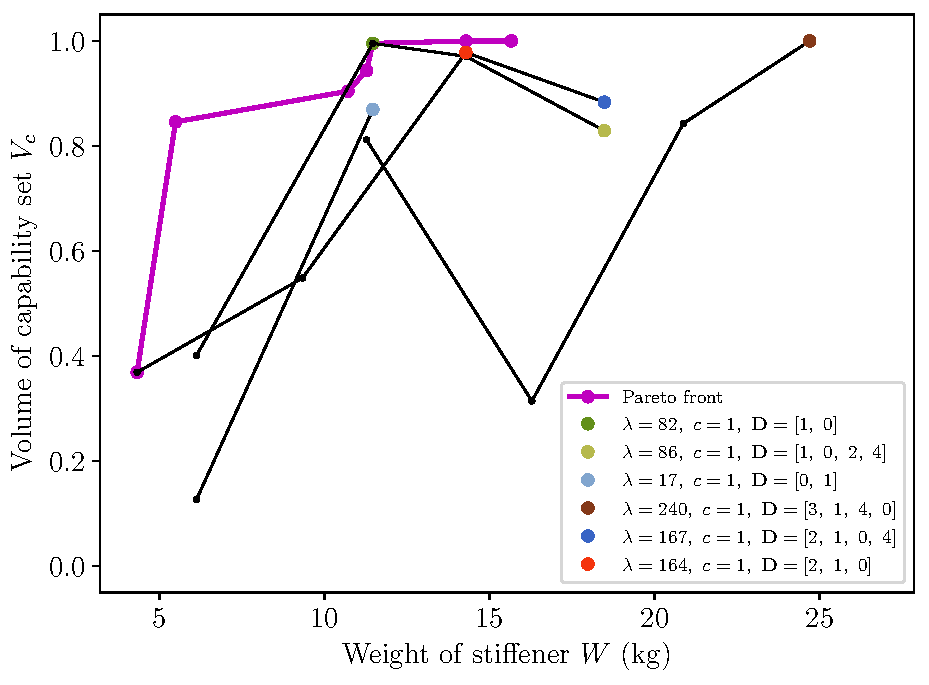
\includegraphics[width=0.5\textwidth]{14a_tradespace_pareto_E_reduced}}
	%
	\subfloat[$S_W$\label{fig:reducedTSE_SW}]{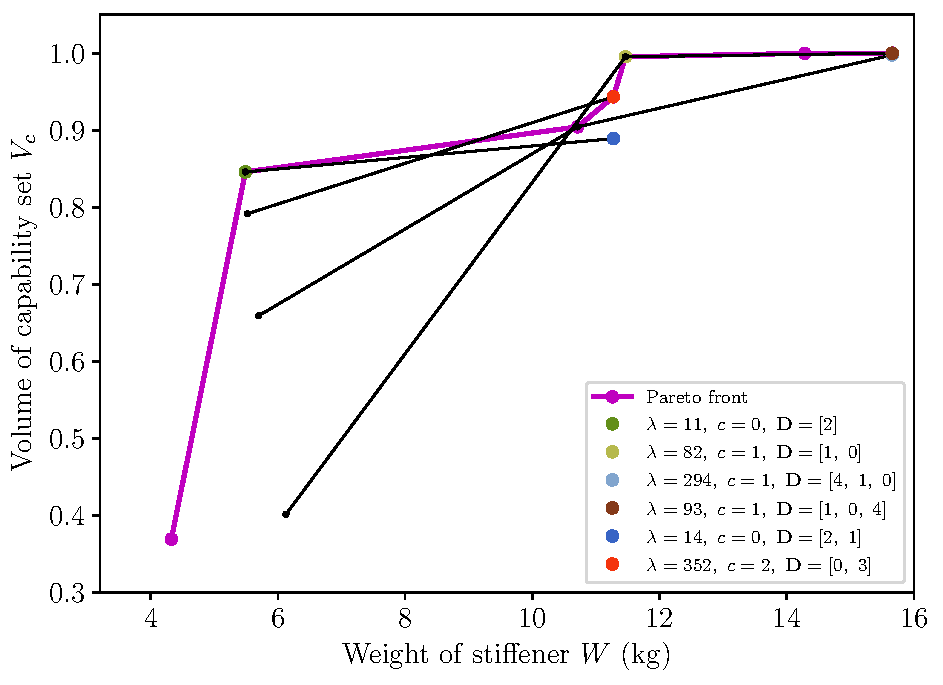
\includegraphics[width=0.5\textwidth]{15a_tradespace_pareto_W_reduced}}
	\caption{Reduced tradespace of solutions in sets $S_E$ and $S_W$}
	\label{fig:reducedTSE}
\end{figure}

Figure~\ref{fig:reducedTSE_SE} and Table~\ref{table:depositionsequence_SE} show that the top 6 designs in $S_E$ share the same concept $c=1$. The top two designs ($\lambda = 82$ and $\lambda = 86$) share the first two deposit choices $D_1=1$ and $D_2=0$. The runner-up design ($\lambda = 86$) adds two additional deposits to the top ranked design ($\lambda = 82$). From Figure~\ref{fig:reducedTSE_SE}, it can be seen that the addition of two more deposits to the top ranked design reduced the capability $V_c$. This is because of the overstiffening of the \ac{TRS} outercasing by the addition of more stiffeners. This overstiffening reduced the fatigue life of the outercasing by inducing concentrated tensile stresses in the unreinforced gaps between the stiffener deposits. The third ranked design ($\lambda = 17$) is identical in geometry to the top ranked designs as seen in Table~\ref{table:depositionsequence_SE} but has the order of the deposit choices interchanged. The discrepancy between $\lambda = 17$ and $\lambda = 82$ is due to the difference in thermomechanical effect of depositing $D_1=0$ first instead of $D_1=1$.

Similar observations can be seen for set $S_W$ in Figure~\ref{fig:reducedTSE_SW}. However, the top performing design belonged to concept $c=0$ while the 6th ranked design belonged to concept $c=2$. Furthermore, the number of deposits used for any given design arc did not exceed $o=3$. In contrast, $S_E$ featured many designs with $o=4$. The fewer number of deposits in $S_W$ can be attributed to the preference of the algorithm for minimizing weight above all. Another difference between $S_W$ and $S_E$ is that most designs in $S_W$ are Pareto optimal as given by the proximity metric in Table~\ref{table:convexhullresults}. $S_W$ has a Pareto proximity metric of $0.0432$ units which is smaller than the value of $0.0904$ units belonging to $S_E$. This is due to the reasons explained earlier regarding the discrepancy between the weight (or cost) and excess. 

% We can see that some of the top performing design arcs are sometimes children of a better performing parent design arc. This is the case with design arc $\lambda = 17$ being the parent of $\lambda = 28$ although $\lambda = 17$ is higher up the ranking within $S_E$. 

\newcommand{\resultsCW}{1.7cm}
\newcommand{\dARA}{\includegraphics[height=1.7cm]{table_E_results/C1D1.pdf}}
\newcommand{\dBRA}{\includegraphics[height=1.7cm]{table_E_results/C1D10.pdf}}

\newcommand{\dARB}{\includegraphics[height=1.7cm]{table_E_results/C1D1.pdf}}
\newcommand{\dBRB}{\includegraphics[height=1.7cm]{table_E_results/C1D10.pdf}}
\newcommand{\dCRB}{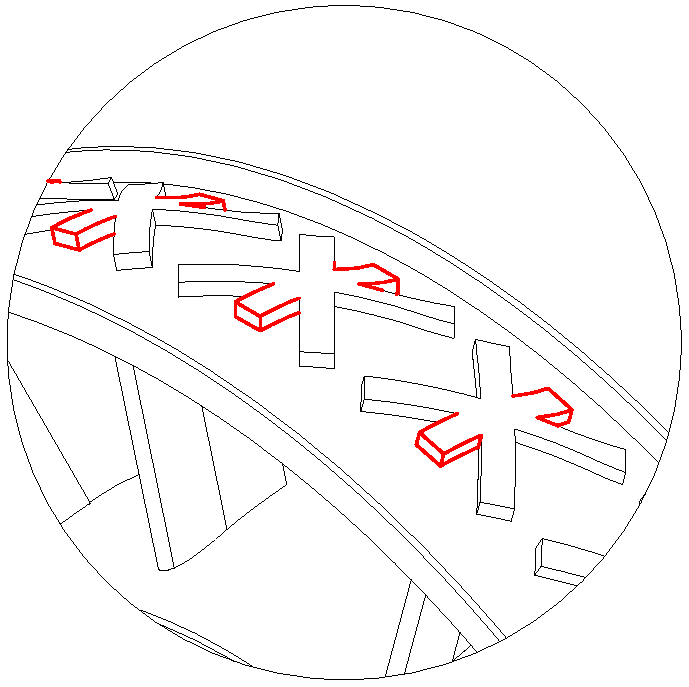
\includegraphics[height=1.7cm]{table_E_results/C1D102.pdf}}
\newcommand{\dDRB}{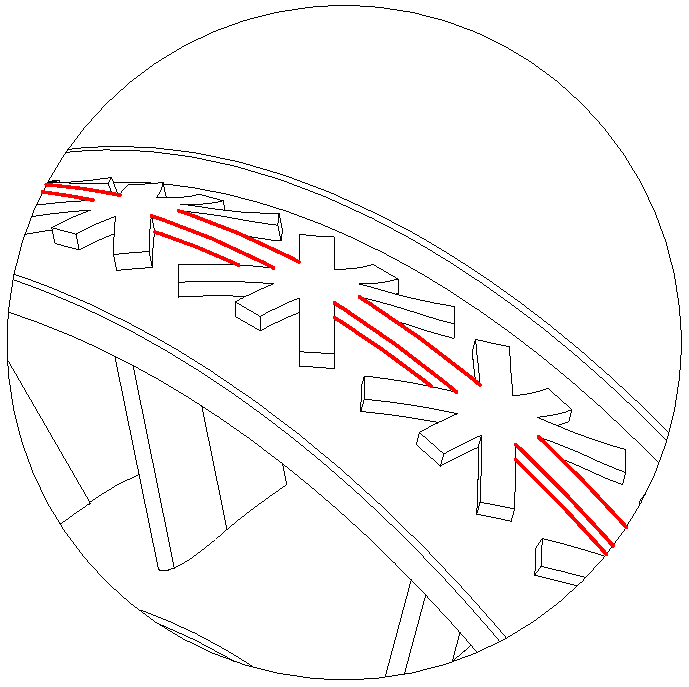
\includegraphics[height=1.7cm]{table_E_results/C1D1024.pdf}}

\newcommand{\dARC}{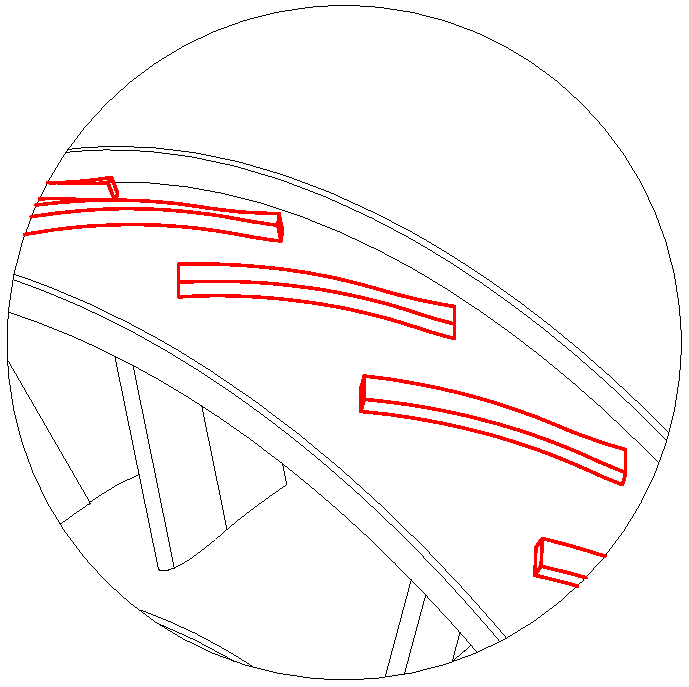
\includegraphics[height=1.7cm]{table_E_results/C1D0.pdf}}
\newcommand{\dBRC}{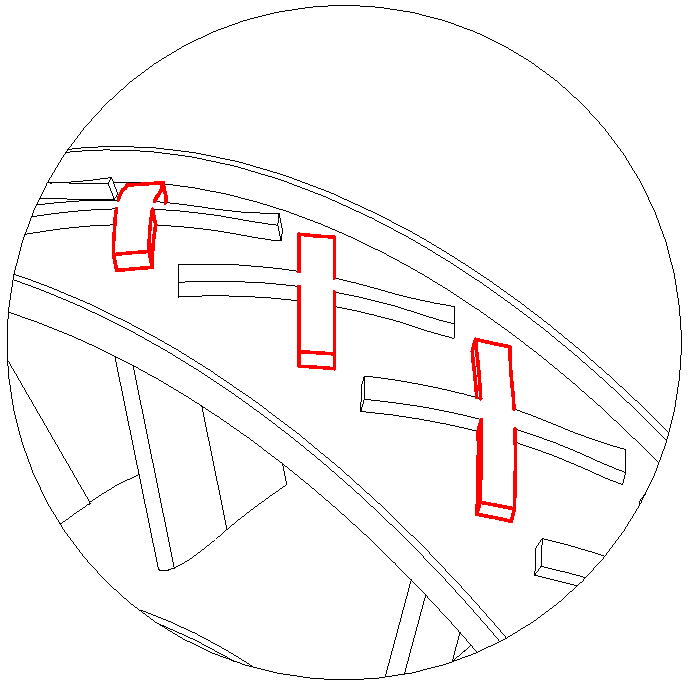
\includegraphics[height=1.7cm]{table_E_results/C1D01.pdf}}

\newcommand{\dARD}{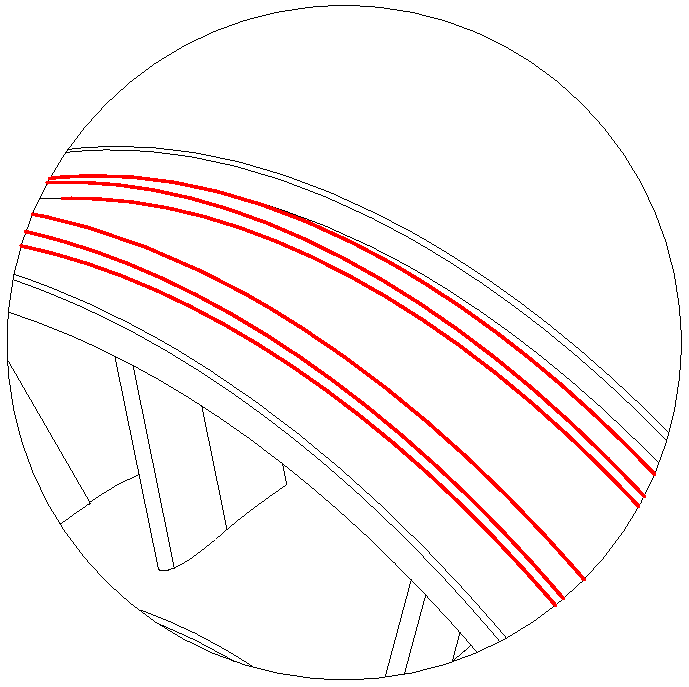
\includegraphics[height=1.7cm]{table_E_results/C1D3.pdf}}
\newcommand{\dBRD}{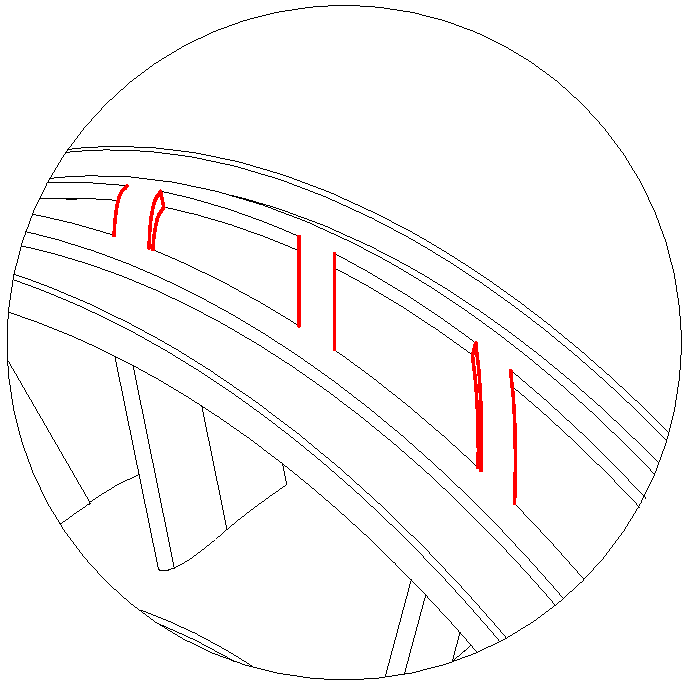
\includegraphics[height=1.7cm]{table_E_results/C1D31.pdf}}
\newcommand{\dCRD}{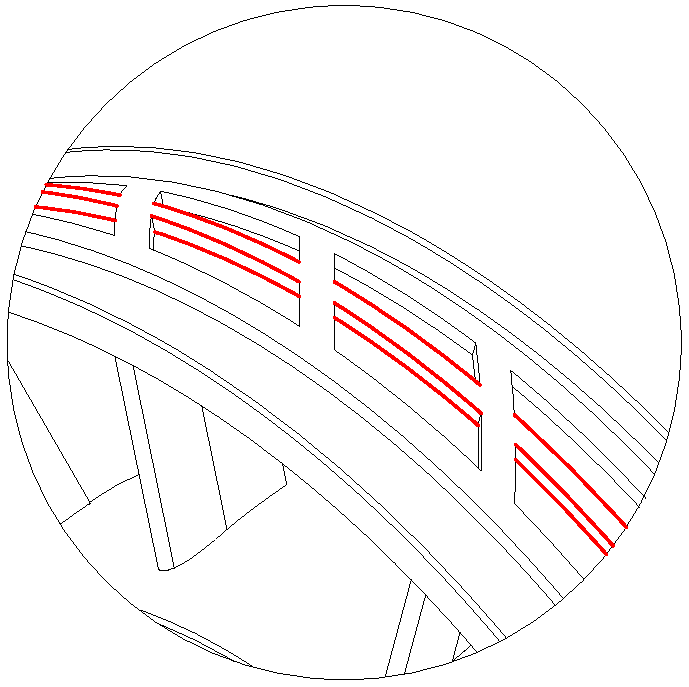
\includegraphics[height=1.7cm]{table_E_results/C1D314.pdf}}
\newcommand{\dDRD}{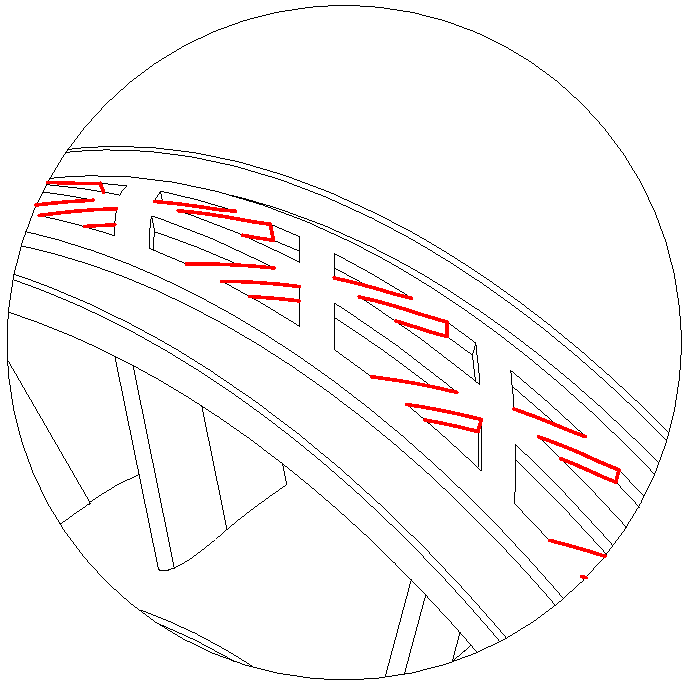
\includegraphics[height=1.7cm]{table_E_results/C1D3140.pdf}}

\newcommand{\dARE}{\includegraphics[height=1.7cm]{table_E_results/C1D2.pdf}}
\newcommand{\dBRE}{\includegraphics[height=1.7cm]{table_E_results/C1D21.pdf}}
\newcommand{\dCRE}{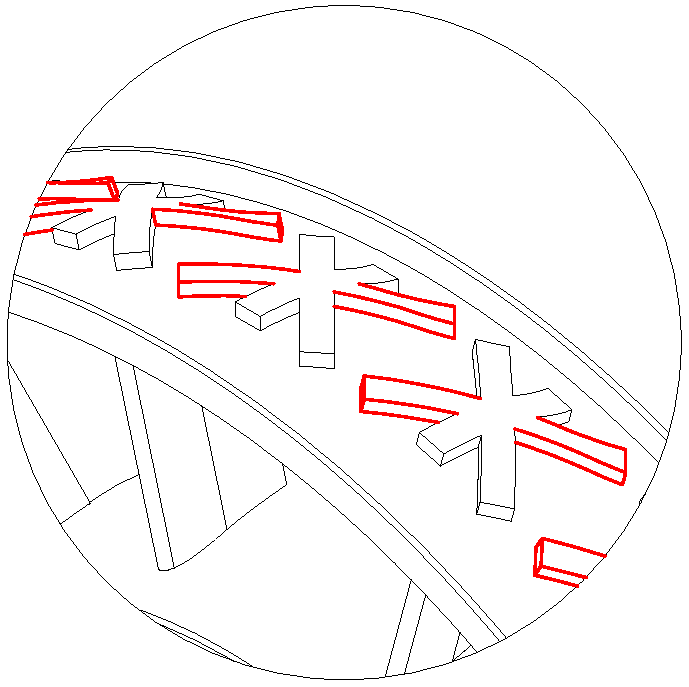
\includegraphics[height=1.7cm]{table_E_results/C1D210.pdf}}
\newcommand{\dDRE}{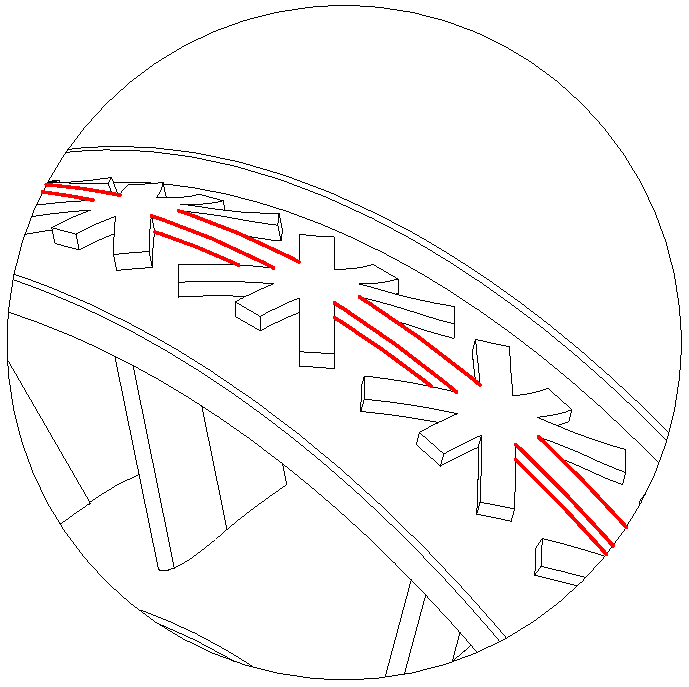
\includegraphics[height=1.7cm]{table_E_results/C1D2104.pdf}}

\newcommand{\dARF}{\includegraphics[height=1.7cm]{table_E_results/C1D2.pdf}}
\newcommand{\dBRF}{\includegraphics[height=1.7cm]{table_E_results/C1D21.pdf}}
\newcommand{\dCRF}{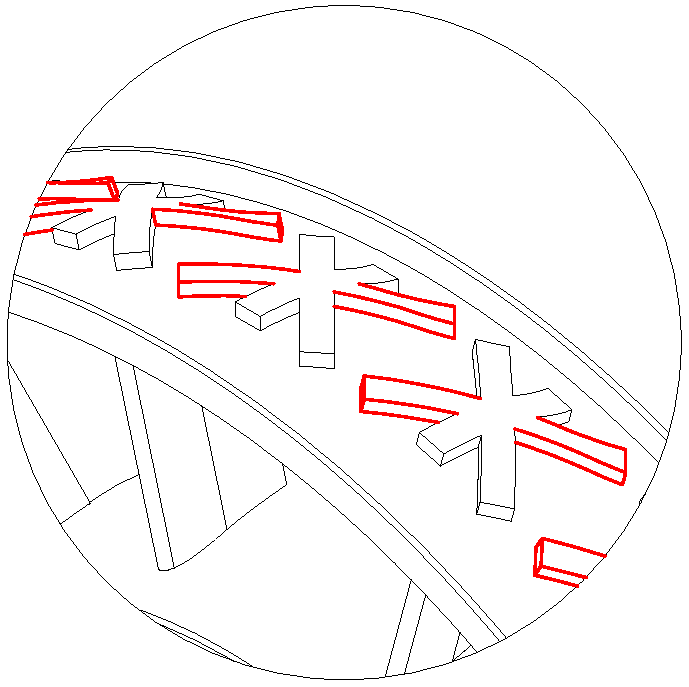
\includegraphics[height=1.7cm]{table_E_results/C1D210.pdf}}

\begin{table}[h!]
	\centering
	\renewcommand{\arraystretch}{1.0}% Wider
	\footnotesize\addtolength{\tabcolsep}{-5pt}
	\caption{Top performing design arcs in $S_E$ detailed annotation}
	\label{table:depositionsequence_SE}
	\begin{tabular}{>{\centering\arraybackslash}m{\resultsCW}>{\centering\arraybackslash}m{\resultsCW}>{\centering\arraybackslash}m{\resultsCW}>{\centering\arraybackslash}m{\resultsCW}>{\centering\arraybackslash}m{\resultsCW}>{\centering\arraybackslash}m{\resultsCW}>{\centering\arraybackslash}m{\resultsCW}}
	\hline\hline

	\bf Design arc Index & \bf concept & \bf 1st deposit & \bf 2nd deposit & \bf 3rd deposit & \bf 4th deposit & \bf 5th deposit \\
	$\lambda$ & $c$ & $D_1$ & $D_2$ & $D_3$ & $D_4$ & $D_5$\\ \hline
	%================================================================
	82 & 1 & \dARA & \dBRA & & & \\ 
	86 & 1 & \dARB & \dBRB & \dCRB & \dDRB & \\
	17 & 1 & \dARC & \dBRC & & & \\ 
	240 & 1 & \dARD & \dBRD & \dCRD & \dDRD & \\ 
	167 & 1 & \dARE & \dBRE & \dCRE & \dDRE & \\
	164 & 1 & \dARF & \dBRF & \dCRF & & \\
	%================================================================
	\hline\hline
	\end{tabular}
\end{table}

\renewcommand{\resultsCW}{1.7cm}
\renewcommand{\dARA}{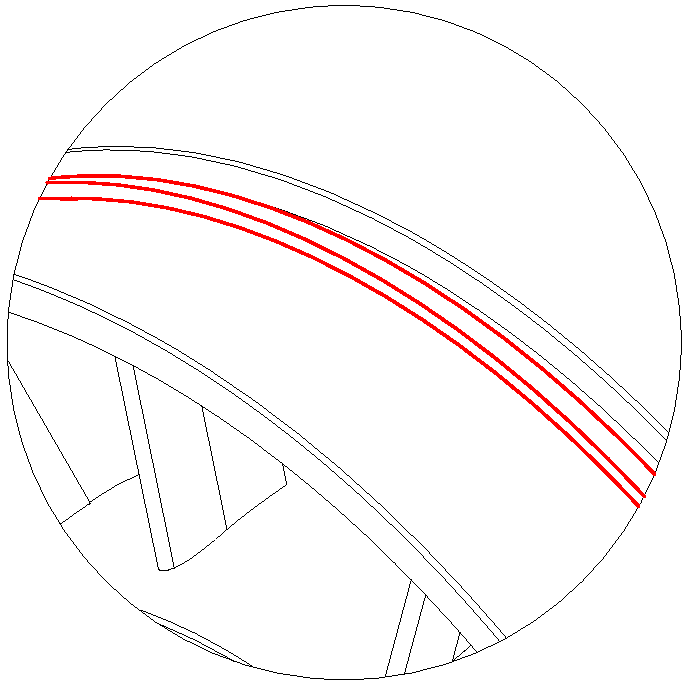
\includegraphics[height=1.7cm]{table_W_results/C0D2.pdf}}

\renewcommand{\dARB}{\includegraphics[height=1.7cm]{table_W_results/C1D1.pdf}}
\renewcommand{\dBRB}{\includegraphics[height=1.7cm]{table_W_results/C1D10.pdf}}

\renewcommand{\dARC}{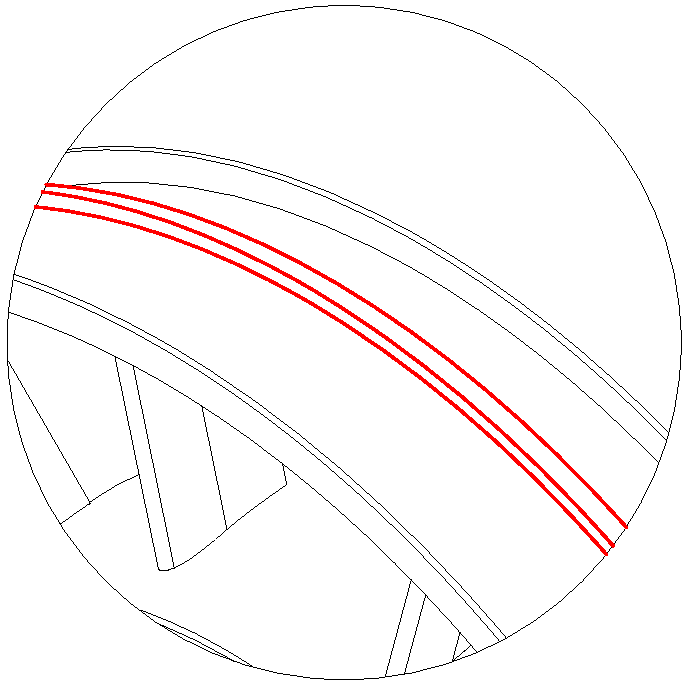
\includegraphics[height=1.7cm]{table_W_results/C1D4.pdf}}
\renewcommand{\dBRC}{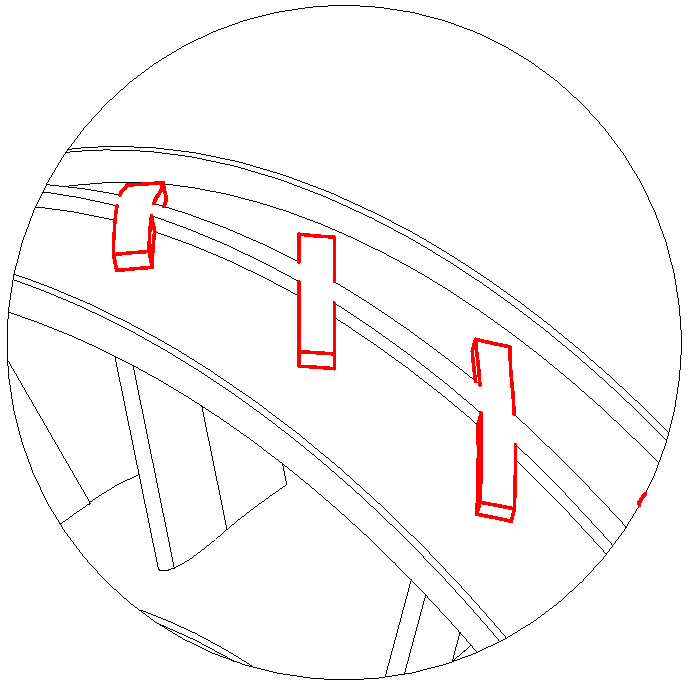
\includegraphics[height=1.7cm]{table_W_results/C1D41.pdf}}
\newcommand{\dCRC}{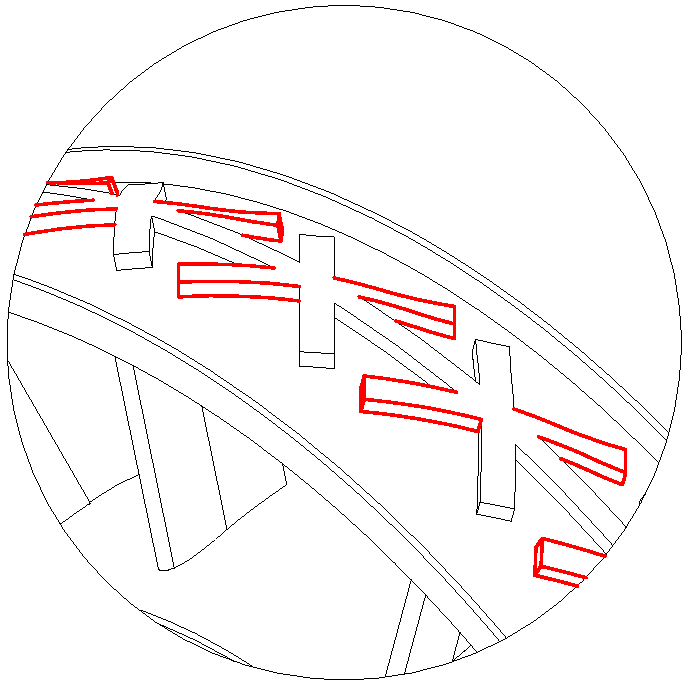
\includegraphics[height=1.7cm]{table_W_results/C1D410.pdf}}

\renewcommand{\dARD}{\includegraphics[height=1.7cm]{table_W_results/C1D1.pdf}}
\renewcommand{\dBRD}{\includegraphics[height=1.7cm]{table_W_results/C1D10.pdf}}
\renewcommand{\dCRD}{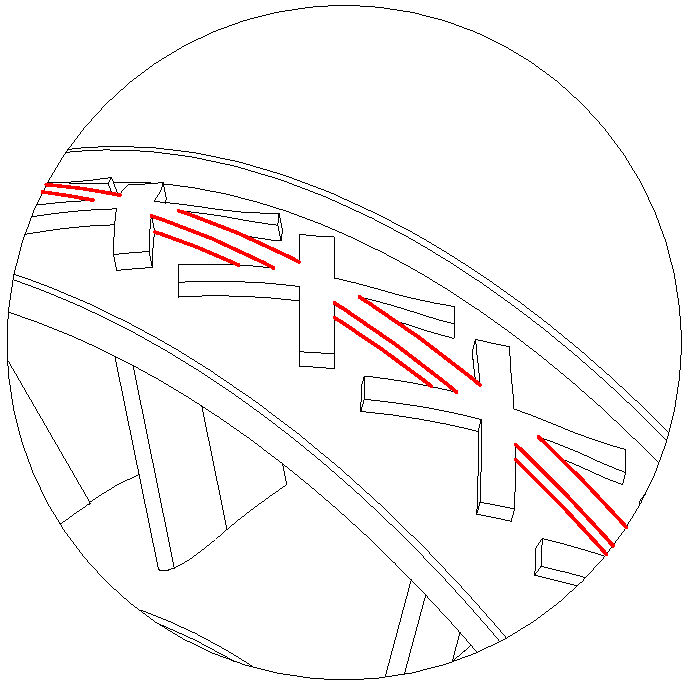
\includegraphics[height=1.7cm]{table_W_results/C1D104.pdf}}

\renewcommand{\dARE}{\includegraphics[height=1.7cm]{table_W_results/C1D2.pdf}}
\renewcommand{\dBRE}{\includegraphics[height=1.7cm]{table_W_results/C1D21.pdf}}

\renewcommand{\dARF}{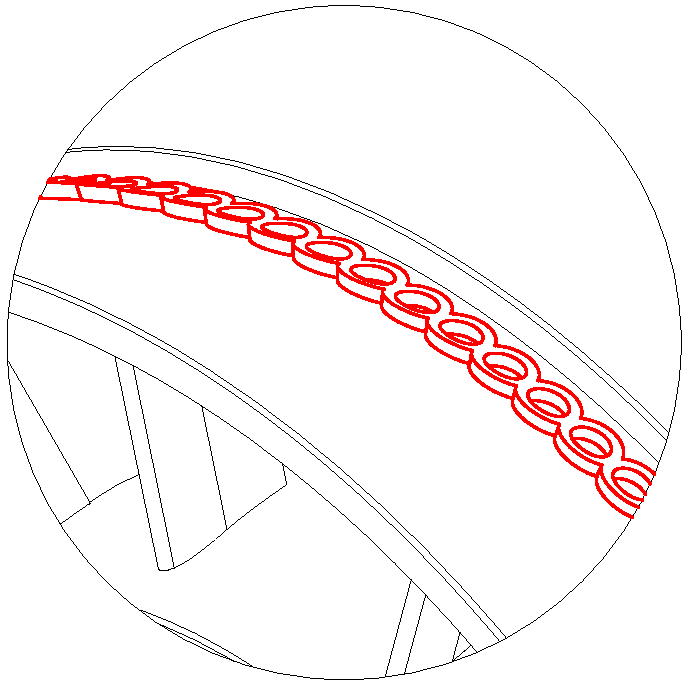
\includegraphics[height=1.7cm]{table_W_results/C2D0.pdf}}
\renewcommand{\dBRF}{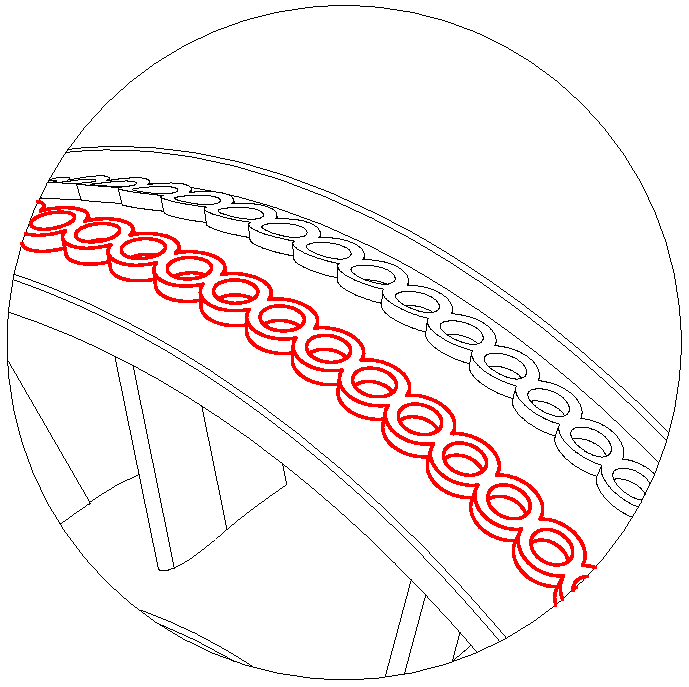
\includegraphics[height=1.7cm]{table_W_results/C2D03.pdf}}

\begin{table}[h!]
	\centering
	\renewcommand{\arraystretch}{1.0}% Wider
	\footnotesize\addtolength{\tabcolsep}{-5pt}
	\caption{Top performing design arcs in $S_W$ detailed annotation}
	\label{table:depositionsequence_SW}
	\begin{tabular}{>{\centering\arraybackslash}m{\resultsCW}>{\centering\arraybackslash}m{\resultsCW}>{\centering\arraybackslash}m{\resultsCW}>{\centering\arraybackslash}m{\resultsCW}>{\centering\arraybackslash}m{\resultsCW}>{\centering\arraybackslash}m{\resultsCW}>{\centering\arraybackslash}m{\resultsCW}}
	\hline\hline

	\bf Design arc Index & \bf concept & \bf 1st deposit & \bf 2nd deposit & \bf 3rd deposit & \bf 4th deposit & \bf 5th deposit \\
	$\lambda$ & $c$ & $D_1$ & $D_2$ & $D_3$ & $D_4$ & $D_5$\\ \hline
	%================================================================
	11 & 0 & \dARA & & & & \\ 
	82 & 1 & \dARB & \dBRB & & & \\
	294 & 1 & \dARC & \dBRC & \dCRC & & \\ 
	93 & 1 & \dARD & \dBRD & \dCRD & & \\ 
	14 & 1 & \dARE & \dBRE & & & \\
	352 & 2 & \dARF & \dBRF & & & \\
	%================================================================
	\hline\hline
	\end{tabular}
\end{table}

\begin{figure}[h!]
	\centering
	\subfloat[$S_E$\label{fig:piechart_concept_SE}]{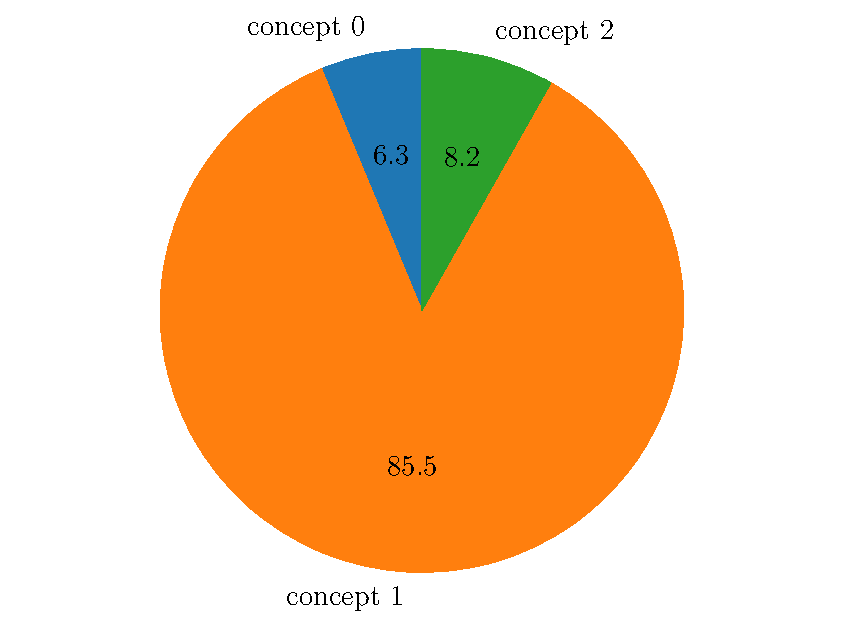
\includegraphics[width=0.5\textwidth]{14c_concept_pie_chart_E}} 
	%
	\subfloat[$S_W$\label{fig:piechart_concept_SW}]{\includegraphics[width=0.5\textwidth]{15c_concept_pie_chart_W}} 
	\caption{Distribution of concepts in sets $S_E$ and $S_W$}
	\label{fig:piechart_concept}
\end{figure}

We analyze the distribution of the concept choices $c$ within the set $S_E$ in Figure \ref{fig:piechart_concept_SE}. We can see that concept choice $c=1$ dwarfs the other two concept choices. This is because the "hatched" concept has deposit choices with relatively high capability and excess. The discontinuous stiffener design featured by its various deposits provided sufficient reinforcement without overstiffening the outercasing. This contrasts the deposit choices available to the "wavy" and "tubular" stiffener concepts which are continuous.

We also look at the distribution of concept choices $c$ within the set $S_W$ in Figure~\ref{fig:piechart_concept_SW}. Two concept choices, $c=0$ and $c=1$ are comparable in terms of frequency within the set. This is because both concepts contain deposit choices that are low in weight. Since the optimization objective for set $S_W$ is weight, the low-weight deposit choices within these concepts are equally preferred.

\begin{figure}[h!]
	\centering
	\subfloat[$S_E$\label{fig:piechart_D1_SE}]{\includegraphics[width=0.5\textwidth]{14b_1st_stage_pie_E}} 
	%
	\subfloat[$S_W$\label{fig:piechart_D1_SW}]{\includegraphics[width=0.5\textwidth]{15b_1st_stage_pie_W}} 
	\caption{Distribution of first deposit $D_1$ when concept $c=1$ is selected in sets $S_E$ and $S_W$}
	\label{fig:piechart_D1}
\end{figure}

We then analyze the distribution of the first choice $D_1$ in the design arcs within the set $S_E$. This distribution is shown in Figure~\ref{fig:piechart_D1_SE}. We can see from this distribution that the redesign choice $D_1 = 1$ is chosen most frequently due the high capability $V_c$ of this deposit choice and its children. The third most common design choice is $D_1 = 0$ which is comparable in frequency to $D_1 = 2$. However, it should be noted that committing to $D_1 = 0$ restricts the designers' choices later in the product's cycle. Figure~\ref{fig:reducedTSE_SE} shows that $\lambda = 17$ is the only possible design arc with $D_1 = 0$. This is in contrast to $D_1 = 1$ that can be used to obtain two different design arcs $\lambda = 82$ and $\lambda = 86$. These additional insights obtained by close examination of the tradespace can be beneficial as opposed to picking the most obvious result from Figure~\ref{fig:piechart_D1}.

The tools developed in this chapter can help designers make informed decisions about the sequence of redesign choices during a product cycle. These insights are particularly useful for determining the first redesign choice when uncertainty is high and the number of possible choices is at its maximum.

%============================== SUMMARY ================================%
\section{Summary}
\label{sec:TSEcontsummary}

This chapter presented a set-based design tool for generating optimal redesign sequences for a product as its lifecycle or development process progresses. These sequences of design choices are represented by design arcs and are obtained by solving a combinatorial optimization problem such that reliability constraints governed by the uncertain requirements are satisfied. The cost function used in optimization is based on the level of excess embedded in a design. 

We mathematically formulate a novel tool for quantifying the level of excess in a design when multiple uncertain parameters are considered simultaneously. Regions of the multi-dimensional parameters space are classified into design capability, requirements, excess or buffer by using a surrogate model. The volume of these sets is obtained via Monte Carlo integration in order to alleviate the curse of dimensionality when considering multi-dimensional problems.

By minimizing the volume of the excess set for a particular design and requirement, overdesign costs are mitigated. We vary the requirements using Monte Carlo simulation with importance sampling to generate requirement arcs. The optimization problem is solved for each requirement arc to obtain a set of corresponding design arcs. 

Tradespace exploration is used to visualize the set of optimal design arcs and compare it to sets of flexible and robust design arcs. Tradespace exploration showed that our approach results in a set of design arcs that balance flexibility and robustness. An examination of the frequency of each design choice within the set of parametric optimal design arcs provides designers with useful insights about the best approach at the early stages of the product's lifecycle or development process when uncertainty is high and decisions have a lasting impact on the product's performance for the remainder of its lifecycle.

The work in this chapter extends the approach used in Chapter~\ref{ch:scalableSBD} to include problems where multiple changes in requirements may occur. This is represented by the requirement arcs discussed in this chapter. Furthermore, robustness in addition to flexibility was quantified and used as a design metric in this chapter.

In the next chapter, we discuss the use of stochastic optimization algorithms for obtaining sets of design solutions when uncertain parameters govern the design optimization problem. Such approaches can help address the need for extensive exploration of the parameters space or the set of possible requirements (given by $\Omega_R$) by reducing the number of needed function evaluations. We show how such approaches can substitute parts of the algorithms that have been developed in this chapter and Chapter~\ref{ch:scalableSBD}.